
%%%%%%%%%%%%%%%%%%%%%%%%%%%%%%%%%%%%%%%%%%%%%%%%%%%%%%%%%%%%%%%%%%%%%
%% This is a (brief) model paper using the achemso class
%% The document class accepts keyval options, which should include
%% the target journal and optionally the manuscript type.
%%%%%%%%%%%%%%%%%%%%%%%%%%%%%%%%%%%%%%%%%%%%%%%%%%%%%%%%%%%%%%%%%%%%%
\documentclass[journal=jctcce,manuscript=article]{achemso}
\setkeys{acs}{articletitle=true}
%%%%%%%%%%%%%%%%%%%%%%%%%%%%%%%%%%%%%%%%%%%%%%%%%%%%%%%%%%%%%%%%%%%%%
%% Place any additional packages needed here.  Only include packages
%% which are essential, to avoid problems later.
%%%%%%%%%%%%%%%%%%%%%%%%%%%%%%%%%%%%%%%%%%%%%%%%%%%%%%%%%%%%%%%%%%%%%
\usepackage{chemformula} % Formula subscripts using \ch{}
\usepackage[T1]{fontenc} % Use modern font encodings
\usepackage{lmodern}
\usepackage{amsmath,amssymb}
\usepackage{graphicx}
\usepackage{float}
\usepackage{braket}
\usepackage{multirow}
\usepackage{array}
\newcolumntype{R}{>{$}r<{$}}
\newcolumntype{C}{>{$}c<{$}}

% Comments
\usepackage[normalem]{ulem}

%%%%%%%%%%%%%%%%%%%%%%%%%%%%%%%%%%%%%%%%%%%%%%%%%%%%%%%%%%%%%%%%%%%%%
%% If issues arise when submitting your manuscript, you may want to
%% un-comment the next line.  This provides information on the
%% version of every file you have used.
%%%%%%%%%%%%%%%%%%%%%%%%%%%%%%%%%%%%%%%%%%%%%%%%%%%%%%%%%%%%%%%%%%%%%
%%\listfiles

%%%%%%%%%%%%%%%%%%%%%%%%%%%%%%%%%%%%%%%%%%%%%%%%%%%%%%%%%%%%%%%%%%%%%
%% Place any additional macros here.  Please use \newcommand* where
%% possible, and avoid layout-changing macros (which are not used
%% when typesetting).
%%%%%%%%%%%%%%%%%%%%%%%%%%%%%%%%%%%%%%%%%%%%%%%%%%%%%%%%%%%%%%%%%%%%%
\newcommand{\x}{{\mathbf{r}}}
\newlength{\dhatheight}
\newcommand{\doublehat}[1]{%
    \settoheight{\dhatheight}{\ensuremath{\hat{#1}}}%
    \addtolength{\dhatheight}{-0.35ex}%
    \hat{\vphantom{\rule{1pt}{\dhatheight}}%
    \smash{\hat{#1}}}}

\newcommand*\mycommand[1]{\texttt{\emph{#1}}}
\newcommand{\filipp}[1]{{\color{red} #1}}
\newcommand{\guo}[1]{{\color{blue} #1}}
\newcommand{\brian}[1]{{\color{orange} #1}}
\newcommand{\eva}[1]{{\color{green} #1}}
%%%%%%%%%%%%%%%%%%%%%%%%%%%%%%%%%%%%%%%%%%%%%%%%%%%%%%%%%%%%%%%%%%%%%
%% Meta-data block
%% ---------------
%% Each author should be given as a separate \author command.
%%
%% Corresponding authors should have an e-mail given after the author
%% name as an \email command. Phone and fax numbers can be given
%% using \phone and \fax, respectively; this information is optional.
%%
%% The affiliation of authors is given after the authors; each
%% \affiliation command applies to all preceding authors not already
%% assigned an affiliation.
%%
%% The affiliation takes an option argument for the short name.  This
%% will typically be something like "University of Somewhere".
%%
%% The \altaffiliation macro should be used for new address, etc.
%% On the other hand, \alsoaffiliation is used on a per author basis
%% when authors are associated with multiple institutions.
%%%%%%%%%%%%%%%%%%%%%%%%%%%%%%%%%%%%%%%%%%%%%%%%%%%%%%%%%%%%%%%%%%%%%
\author{Brian D. Nguyen}
\author{Guo P. Chen}
\author{Matthew M. Agee}
\author{Asbj{\"o}rn M. Burow}
\author{Matthew P. Tang}
\author{Filipp Furche}
\affiliation{Department of Chemistry, University of California, Irvine,
    1102 Natural Sciences II, Irvine, CA 92697-2025, USA}
\email{filipp.furche@uci.edu}
%%%%%%%%%%%%%%%%%%%%%%%%%%%%%%%%%%%%%%%%%%%%%%%%%%%%%%%%%%%%%%%%%%%%%
%% The document title should be given as usual. Some journals require
%% a running title from the author: this should be supplied as an
%% optional argument to \title.
%%%%%%%%%%%%%%%%%%%%%%%%%%%%%%%%%%%%%%%%%%%%%%%%%%%%%%%%%%%%%%%%%%%%%
\title[RPA]{Divergence of Many-Body Perturbation Theory for Noncovalent
  Interactions of Large Molecules}
%  {Size dependence of noncovalent interactions within the random
%     phase approximation}

%%%%%%%%%%%%%%%%%%%%%%%%%%%%%%%%%%%%%%%%%%%%%%%%%%%%%%%%%%%%%%%%%%%%%
%% Some journals require a list of abbreviations or keywords to be
%% supplied. These should be set up here, and will be printed after
%% the title and author information, if needed.
%%%%%%%%%%%%%%%%%%%%%%%%%%%%%%%%%%%%%%%%%%%%%%%%%%%%%%%%%%%%%%%%%%%%%
% \abbreviations{IR,NMR,UV}
\keywords{RPA, Dispersion, Perturbation Method}

%%%%%%%%%%%%%%%%%%%%%%%%%%%%%%%%%%%%%%%%%%%%%%%%%%%%%%%%%%%%%%%%%%%%%
%% The manuscript does not need to include \maketitle, which is
%% executed automatically.
%%%%%%%%%%%%%%%%%%%%%%%%%%%%%%%%%%%%%%%%%%%%%%%%%%%%%%%%%%%%%%%%%%%%%
\begin{document}

%%%%%%%%%%%%%%%%%%%%%%%%%%%%%%%%%%%%%%%%%%%%%%%%%%%%%%%%%%%%%%%%%%%%%
%% The "tocentry" environment can be used to create an entry for the
%% graphical table of contents. It is given here as some journals
%% require that it is printed as part of the abstract page. It will
%% be automatically moved as appropriate.
%%%%%%%%%%%%%%%%%%%%%%%%%%%%%%%%%%%%%%%%%%%%%%%%%%%%%%%%%%%%%%%%%%%%%
\begin{tocentry}

% Some journals require a graphical entry for the Table of Contents.
% This should be laid out ``print ready'' so that the sizing of the
% text is correct.

% Inside the \texttt{tocentry} environment, the font used is Helvetica
% 8\,pt, as required by \emph{Journal of the American Chemical
% Society}.

% The surrounding frame is 9\,cm by 3.5\,cm, which is the maximum
% permitted for  \emph{Journal of the American Chemical Society}
% graphical table of content entries. The box will not resize if the
% content is too big: instead it will overflow the edge of the box.

% This box and the associated title will always be printed on a
% separate page at the end of the document.

  \centering
  
\includegraphics{ni_toc.eps}

\end{tocentry}


%%%%%%%%%%%%%%%%%%%%%%%%%%%%%%%%%%%%%%%%%%%%%%%%%%%%%%%%%%%%%%%%%%%%%
%% The abstract environment will automatically gobble the contents
%% if an abstract is not used by the target journal.
%%%%%%%%%%%%%%%%%%%%%%%%%%%%%%%%%%%%%%%%%%%%%%%%%%%%%%%%%%%%%%%%%%%%%


\begin{abstract}
  Prompted by recent reports of large errors in noncovalent interaction (NI)
  energies obtained from many-body perturbation theory (MBPT), we compare the
  performance of second-order M{\o}ller--Plesset MBPT (MP2), spin-scaled MP2,
  dispersion-corrected semilocal density functional approximations (DFA), and
  the post-Kohn--Sham random phase approximation (RPA) for predicting
  binding energies of supramolecular complexes contained in the S66, L7,
  and S30L benchmarks. All binding energies are extrapolated
  to the basis set limit, corrected for basis set superposition
  errors, and compared to reference results of the domain-based local pair-natural
  orbital coupled-cluster (DLPNO-CCSD(T)) or better quality. Our results confirm
  that MP2 severely overestimates binding energies of large complexes,
  producing relative errors of over 100\% for several benchmark
  compounds. RPA relative errors  
  consistently range between 5-10\%, significantly less than reported
  previously using smaller basis sets, whereas spin-scaled MP2 methods
  show limitations similar to MP2, albeit less pronounced, and empirically
  dispersion-corrected DFAs perform almost as well as RPA. Regression
  analysis reveals a systematic increase of relative MP2 binding energy
  errors with the system size at a rate of approximately 0.1$\%$
  per valence electron, whereas the RPA and
  dispersion-corrected 
  DFA relative errors are virtually independent of the system
  size. These observations are corroborated by a comparison of
  computed rotational constants of organic molecules to gas-phase
  spectroscopy data contained in the ROT34 benchmark. To analyze these
  results, an asymptotic adiabatic
  connection symmetry-adapted perturbation theory (AC-SAPT) is
  developed which uses monomers at full coupling whose ground-state density is
  constrained to the ground-state density of the complex. Using the
  fluctuation--dissipation theorem, we obtain a 
  nonperturbative ``screened second-order'' expression for the
  dispersion energy in terms of 
  monomer quantities which is exact for non-overlapping subsystems and
  free of induction terms;
  a first-order RPA-like approximation to the Hartree, exchange, and
  correlation kernel recovers the macroscopic Lifshitz limit. The
  AC-SAPT expansion of the interaction energy is obtained from Taylor
  expansion of the coupling strength integrand.
  Explicit
  expressions for the convergence radius of the AC-SAPT series are derived
  within RPA and MBPT and numerically evaluated. Whereas the AC-SAPT
  expansion is always convergent for nondegenerate monomers when RPA is used,
  it is found to spuriously diverge for second-order MBPT, except for
  the smallest and 
  least polarizable monomers. The divergence of the AC-SAPT series within
  MBPT is numerically confirmed within RPA; prior numerical results on
  the convergence of the SAPT expansion for MBPT methods are revisited
  and support this conclusion once sufficiently high orders are
  included. The cause of the 
  failure of MBPT methods for NIs of large systems is missing or
  incomplete ``electrodynamic'' 
  screening of the Coulomb interaction due to induced particle--hole
  pairs between electrons in different
  monomers, leaving the 
  effective interaction too strong for AC-SAPT to 
  converge. Hence, MBPT cannot be considered reliable 
  for quantitative predictions of NIs, even in moderately polarizable
  molecules with 
  a few tens of atoms. The failure to accurately account for
  electrodynamic polarization makes MBPT qualitatively unsuitable for 
  applications such as NIs of nanostructures, macromolecules, and soft
  materials; more robust
  non-perturbative approaches such as RPA or coupled cluster methods
  should be used instead whenever possible.
\end{abstract}

%%%%%%%%%%%%%%%%%%%%%%%%%%%%%%%%%%%%%%%%%%%%%%%%%%%%%%%%%%%%%%%%%%%%%
%% Start the main part of the manuscript here.
%%%%%%%%%%%%%%%%%%%%%%%%%%%%%%%%%%%%%%%%%%%%%%%%%%%%%%%%%%%%%%%%%%%%%
\section{Introduction}

While covalent bonding is a central paradigm of chemical theory,
noncovalent interactions
(NIs)\cite{HobzaCollectCzechChemCommun, Dobson12JPhysCondensMatter24p073201}
are often considered secondary due to their ``weakness.'' For small
molecules with 10 or less atoms, NIs are at least one order of magnitude
smaller than covalent bonds, and 
their low chemical specificity makes them difficult to detect and control.
However, it has long been recognized that NIs 
are pairwise nonadditive and can grow superlinearly with system size.
\cite{DobsonIntJQuantumChem,doi:10.1063/1.1723844,muto1943force}
Indeed, NIs are key factors determining conformation, tertiary
structure, and other 
properties of molecular aggregates and complexes,\cite{Huang16Langmuir32p12352,
  Biedermann16ChemRev116p5216, Britz06ChemSocRev35p637}
materials,\cite{Liu13AdvMater25p1521, Georgakilas16ChemRev116p5464}
or molecular crystals.\cite{Moulton01ChemRev101p1629, 
  Beran16ChemRev116p5567}
Recent advances in experimental techniques such as molecular beam
spectroscopy\cite{Becucci16ChemRev116p5014}
have made NIs readily observable in larger molecular systems, and even
areas focused on  
covalent bonding such as synthetic chemistry and catalysis
increasingly use NIs to fine-tune reactivity and selectivity.
\cite{Zuend09JAmChemSoc131p15358, Tao16ChemEurJ22p8786}

Perhaps with the exception of density functional theory, most electronic
structure methods have been developed and tested for small molecules. A
central assumption underlying this ``bottom-up'' approach is that methods performing well for small
systems may be scaled up to larger ones without deterioration in accuracy.
Size consistency and size extensivity\cite{doi:10.1002/qua.560100802,
  doi:10.1146/annurev.pc.32.100181.002043,hirata2011} 
are often assumed to be sufficient to ensure that the accuracy of an
electronic structure method for chemical processes is approximately
independent of the system size. M{\o}ller--Plesset (MP) many-body
perturbation theory (MBPT),\cite{PhysRev.46.618} 
which is based on the Fock operator as a zeroth-order Hamiltonian, has enjoyed
much popularity as one of the least expensive yet useful ab-initio
correlated electronic methods; size-extensivity of the energy is an
often cited advantage of MP theory \cite{doi:10.1002/qua.560100802}.
Moreover, unlike semilocal density functional approximations (DFAs), whose
performance for NIs can be erratic,\cite{Kristyan94ChemPhysLett229p175,perezJorda1995134,
  doi:10.1002/jcc.540161102} MBPT has widely been considered a
qualitatively suitable starting point for modeling NIs, particularly in
systems too large to be tractable by more advanced
methods.\cite{doi:10.1021/jp070589p,doi:10.1002/cphc.200800718,Riley12JPhysChemA116p4159}
This view appears to have emerged from the correct $1/R^6$ behavior of the
dispersion energy obtained from MBPT as well as early favorable convergence for
small closed-shell systems.\cite{doi:10.1002/qua.560450502,doi:10.1063/1.465554}
In a landmark 1993 paper\cite{doi:10.1002/qua.560450502}, Moszynski,
Jeziorski, and Szalewicz investigated the convergence of the MBPT
expansion of the dispersion energy for several small weakly bound
complexes and concluded that convergence of the series is ``very fast.''
This may be contrasted with covalent interactions, where MBPT is known
to diverge in many systems of chemical interest.\cite{doi:10.1063/1.472352,
  doi:10.1021/jp952815d,doi:10.1063/1.481764}
The assumption that ``weak'' closed-shell interactions between distant electron
pairs are accurately captured by MBPT is implicit in many applications
as well as 
theoretical approaches such as local correlation
methods.\cite{doi:10.1063/1.2982419} Against the backdrop of the
qualitative inability of semilocal DFAs to capture 
long-range NIs, this assumption has also motivated the development of
efficient computational 
methods to apply MBPT to systems with 100 and more atoms.\cite{pulay1983151,doi:10.1063/1.479957,
  doi:10.1063/1.4923369,doi:10.1063/1.1578621,doi:10.1021/acs.jctc.7b00176}

However, with the expanding scope of MBPT applications during the past
two decades, an increasing number of examples were reported that shows
substantial overestimation of NI energies by second-order MP MBPT (MP2).\cite{doi:10.1002/wcms.84}
In 2010, Pulay and co-workers pointed out that MP2 overbinds coronene dimer
by almost 100\% compared to the quadratic configuration interaction reference
data.\cite{doi:10.1080/00268970903397249,doi:10.1007/s00214-011-1009-6}
Comparing initially to solution phase thermodynamic
data\cite{Grimme06JComputChem27p1787} and later to coupled cluster singles, doubles,
and perturbative triples (CCSD(T)) calculations,\cite{doi:10.1063/1.3382344}
Grimme noted  that the accuracy of MP2 severely deteriorates for supramolecular
systems.\cite{Grimme12ChemEurJ18p9955}. Initially, these deviations
were viewed as the result of a quantitative rather than qualitative 
shortcomings of MBPT, which led to the development of empirical correction
schemes such as spin-component-scaled MP2 methods\cite{Grimme03JChemPhys118p9095,doi:10.1063/1.1809602}
and MP2.5.\cite{doi:10.1002/cphc.200800718} For large molecular complexes,
the shortcomings of pairwise additive methods such as MP2 have been ascribed
to missing three- and higher-body dispersion interactions,\cite{Grimme12ChemEurJ18p9955}
triggering the development of dispersion corrections including MP2C,
\cite{doi:10.1063/1.2905808,Pitonak10JChemTheoryComput6p168,doi:10.1063/1.4809981}
MP2D,\cite{doi:10.1021/acs.jctc.8b00548,C9SC05689K} as well as
empirical three-\cite{Grimme12ChemEurJ18p9955,Caldeweyher17JChemPhys147p034112},
and many-body\cite{Tkatchenko12PhysRevLett108p236402} dispersion
corrections for DFAs.
Meanwhile, Dobson and co-workers showed
that the simple addition of pairwise $1/R^6$ interactions 
yields qualitatively incorrect asymptotic power laws for dispersion
interactions between macroscopic solids. For example, the interaction
between two large parallel graphene sheets decays as $1/D^3$ with the
distance $D$ between the sheets, whereas finite-order MBPT yields a
$1/D^4$ behavior.\cite{PhysRevLett.96.073201,Lebegue10PhysRevLett105p196401}
These troubling inconsistencies and the sheer magnitude of the errors
raise the question whether and to what extent MBPT is 
fundamentally adequate for NIs of large but finite molecules.

To address this question, we revisit the performance of MBPT with 
particular emphasis on large molecules with 100 and more atoms, and
contrast it with the random phase approximation (RPA) to the
ground-state correlation 
energy in a density functional context\cite{Langreth75SolidStateCommun17p1425,
Langreth77PhysRevB15p2884,PhysRevB.59.4708}.
Particle--hole RPA may be viewed as a resummation of ring diagrams\cite{PhysRev.106.364}
which correspond to direct Coulomb interactions between particle--hole pairs
and constitute the most long-ranged correlation contribution to the
interaction energy between closed-shell
systems\cite{Dobson05IntJQuantumChem101p579, 
  Dobson12JPhysCondensMatter24p073201}.
Indeed, the accuracy of RPA for NIs in small molecules,\cite{Eshuis11JPhysChemLett2p983,
  doi:10.1063/1.3494541} 
rare-gas solids,\cite{Harl09PhysRevLett103p056401} and layered
materials\cite{Lebegue10PhysRevLett105p196401} 
is well documented, but few results for intra- and intermolecular NIs
in large systems are available.\cite{heelmann201765,doi:10.1063/1.5025938} Building on efficient
RPA implementations for energy\cite{Eshuis10JChemPhys132p234114} and analytic 
derivatives\cite{Burow14JChemTheoryComput10p180}, we investigate the
size-dependence of MBPT and RPA interaction energies using the 
S66,\cite{doi:10.1021/ct2002946,doi:10.1021/ct200523a}
L7,\cite{doi:10.1021/ct400036b} and S30L\cite{Sure15JChemTheoryComput}
benchmarks in Section \ref{sec:results}.
These benchmarks contain systems ranging from 6 to 204 atoms, with
binding energies between 1 kcal/mol and 136 kcal/mol. To evaluate whether our
observations for energetics also hold for structures, we also compare
rotational constants  
from MP2, RPA, and Grimme's dispersion corrected DFA-D3\cite{Grimme12ChemEurJ18p9955}
structure optimizations  to gas-phase spectroscopy data using organic
molecules with 18--35 atoms from the ROT34 benchmark
set\cite{C3CP52293H,Risthaus14JComputChem35p1509}.

In Section \ref{sec:SAPT}, these results are analyzed in detail using a
symmetry-adapted perturbation theory (SAPT) type\cite{doi:10.1080/00268977900101601,
  doi:10.1063/1.461528} 
asymptotic theory of NIs between closed-shell fragments whose
ground-state density is constrained to the supersystem ground-state
density using a local one-body potential in the spirit of the adiabatic
connection (AC)\cite{Langreth77PhysRevB15p2884,Langreth75SolidStateCommun17p1425,  
  PhysRevB.13.4274,PhysRevB.15.6006.3} in density functional
theory (DFT). This leads to a compact, non-perturbative expression for
the dispersion energy, as well as explicit estimates for the convergence
radius of the AC-SAPT expansion. We investigate how the estimated
convergence radii correlate with errors of MP2 and RPA calculations of
NIs and the system size. A numerical model for the divergence of the
AC-SAPT expansion for moderately large and polarizable
systems is obtained by re-expansion of the RPA correlation
energy into powers of the interaction. Conclusions for electronic
structure theory and computational practice are
presented in Sec. \ref{sec:conclusions}.

\section{Methods}
\label{sec:methods}
\subsection{Computational Details}

MP2 energies were evaluated using on self-consistent Hartree--Fock (HF)
orbitals. 
Variants of MP2 such as spin-component-scaled MP2 (SCS-MP2)\cite{Grimme03JChemPhys118p9095}
and scaled opposite-spin MP2 (SOS-MP2)\cite{doi:10.1063/1.1809602} were also assessed.
All MP2 calculations were performed with the RI approximation (RI-MP2)
using the \texttt{ricc2}
module\cite{b515355g} of \textsc{Turbomole}.\cite{Furche14WIREsComputMolSci4p91}

RPA energies and analytic derivatives were obtained in a post-Kohn--Sham
(KS) fashion, i.e., a KS calculation using a semilocal DFA was first performed to
obtain the KS orbitals, and subsequently the exact exchange energy and the RPA
correlation energy were evaluated non-self-consistently. The
Perdew--Burke--Ernzerhof (PBE)\cite{Perdew96PhysRevLett77p3865} and
Tao--Perdew--Staroverov--Scuseria (TPSS)\cite{Tao03PhysRevLett91p146401}
DFAs were used for the KS calculations; the ensuing RPA calculations,
dubbed RPA(PBE) and RPA(TPSS), respectively, employed the
resolution-of-the-identity (RI) approximation and the imaginary frequency
integration technique as implemented in the \texttt{rirpa} module\cite{Eshuis10JChemPhys132p234114}
of \textsc{Turbomole}.\cite{Furche14WIREsComputMolSci4p91}
Perturbative order-by-order analysis of the RPA correlation energies was carried out using 
a modified version of \textsc{Turbomole 7.3}.

Tight convergence criteria of $10^{-9}$ Hartrees for the energy and
$10^{-7}$ atomic units (a.u.) for the root mean square change of the
one-particle density matrix were used for 
the KS and HF self-consistent field iterations. DFA quadrature grids of
m5 quality\cite{Treutler95JChemPhys102p346} were used for the KS
reference calculations. Imaginary frequency grids of 100 points 
were employed for the RPA energy calculations. Interaction energies
were computed based on the supermolecular approach and extrapolated to
the complete basis set (CBS) limit, as detailed in the next subsection.
RPA structural optimizations\cite{Burow14JChemTheoryComput10p180}
of molecules in the ROT34 benchmark set were converged to a maximum
Cartesian gradient norm $\leq 10^{-4}$~a.u. and $10^{-7}$~a.u. in the
energy change. Fine imaginary frequency grids of 200 points were used
for RPA gradient calculations and structure optimizations.

The interaction energies were benchmarked against CCSD(T) values for
the S66 benchmark set\cite{doi:10.1021/ct2002946,doi:10.1021/ct200523a}
and against the domain-based local pair-natural orbital (DLPNO)
based CCSD(T) calculations for the L7 and S30L benchmark
sets.\cite{doi:10.1063/1.5090222,doi:10.1063/1.5012601}
DLPNO-CCSD(T) results can vary significantly for weakly bound
complexes depending on the truncation of the PNO basis and domain
size.\cite{doi:10.1021/ct501129s,doi:10.1021/acs.jpclett.9b01156}
Moreover, even with tight truncation thresholds, the results may
differ by up to $\sim$2 kcal/mol based on the choice of basis set and
basis-set extrapolation scheme as seen by Refs.~\citenum{doi:10.1063/1.5012601}
and \citenum{doi:10.1021/acs.jpclett.9b01156}. For the present study,
the DLPNO-CCSD(T) reference values were taken from Brandenburg
\textit{et al}\cite{doi:10.1063/1.5012601} employing the ``TightPNO''
truncation thresholds\cite{doi:10.1021/ct501129s} and the basis-set extrapolation scheme from
Ref.~\citenum{doi:10.1021/acs.jctc.5b00515}
for both the L7 and S30L benchmarks. Throughout the paper,
signed errors are defined as differences between calculated and
reference values; for example, a positive error in binding
energies signifies underbinding.

\subsection{Basis Set Convergence} \label{sub:basis_set}

The RPA total energy is the sum of the energy expectation value of the
KS determinant, i.e., the sum of the zeroth- and first-order energies, and
the RPA correlation energy. These two parts of the energy exhibit
qualitatively different basis set convergence\cite{Eshuis12JChemPhys136p084105}.
The energy expectation value of the KS determinant was evaluated within
the RI-$JK$ algorithm with the corresponding optimized auxiliary basis
sets.\cite{b204199p} Karlsruhe segmented-contracted polarized
quadruple-$\zeta$ (def2-QZVP) 
basis sets\cite{Weigend05PhysChemChemPhys7p3297,Weigend03JChemPhys119p12753}
were chosen for the KS reference calculations because they were
found to yield 
significantly faster convergence of the KS energy expectation value than
the corresponding correlation-consistent basis sets using generalized
contractions.\cite{Dunning89JChemPhys90p1007,doi:10.1063/1.464303,b415208e} 

RPA correlation energies were evaluated using Dunning's correlation-consistent 
polarized valence basis
sets\cite{Dunning89JChemPhys90p1007,doi:10.1063/1.464303} 
in conjunction with the corresponding auxiliary correlation-consistent basis
sets optimized for RI-MP2.\cite{Weigend02JChemPhys116p3175,b415208e}
Small core relativistic
effective core potentials\cite{doi:10.1063/1.1622924,doi:10.1021/jp065887l}
were used for the halogen atoms in the S30L\cite{Sure15JChemTheoryComput}
benchmark set.
The frozen core approximation was employed for the RPA correlation energy
calculations. Basis set superposition error was estimated by 50\%
counterpoise (CP) correction as recommended by Risthaus and
coworkers;\cite{Risthaus13JChemTheoryComput9p1580} the CP correction was
only applied to the RPA correlation energy.

The CBS limit of the RPA correlation energy was estimated using the two-point
$1/X^3$ extrapolation, where $X = 3$ (triple-$\zeta$), $4$ (quadruple-$\zeta$),
etc.\cite{Eshuis12JChemPhys136p084105,Halkier98ChemicalPhysicsLetters286p243} Dunning's
correlation-consistent polarized triple- (cc-pVTZ) and quadruple-$\zeta$ (cc-pVQZ) valence basis
sets\cite{Dunning89JChemPhys90p1007,doi:10.1063/1.464303} were employed for
the 3-4 extrapolation. The basis set dependence of the S30L interaction
energies is displayed in Figure \ref{fig:conv}. To assess the residual
basis set error, exploratory calculations were performed using Dunning's
cc-pV5Z basis 
sets\cite{b415208e} for the pincer complex with 2,4,7-trinitro-9-fluorenone
as the guest molecule (TNF@tweezer2, compound 5).\cite{Sure15JChemTheoryComput}
The 4-5 extrapolation was found to be within 0.20 kcal/mol compared to
the 3-4 extrapolation, see Figure S1 in the Supporting
Information. 

Similarly, correlation energies from MP2 and its variants were obtained
using the frozen core approximation, $50\%$ CP correction, and the 3-4 extrapolation 
using cc-pVTZ and cc-pVQZ
basis sets.\cite{Dunning89JChemPhys90p1007,doi:10.1063/1.464303}
HF energies were computed using def2-QZVP
basis set.\cite{Weigend05PhysChemChemPhys7p3297,Weigend03JChemPhys119p12753}


\begin{figure}[hbpt]
  \centering
  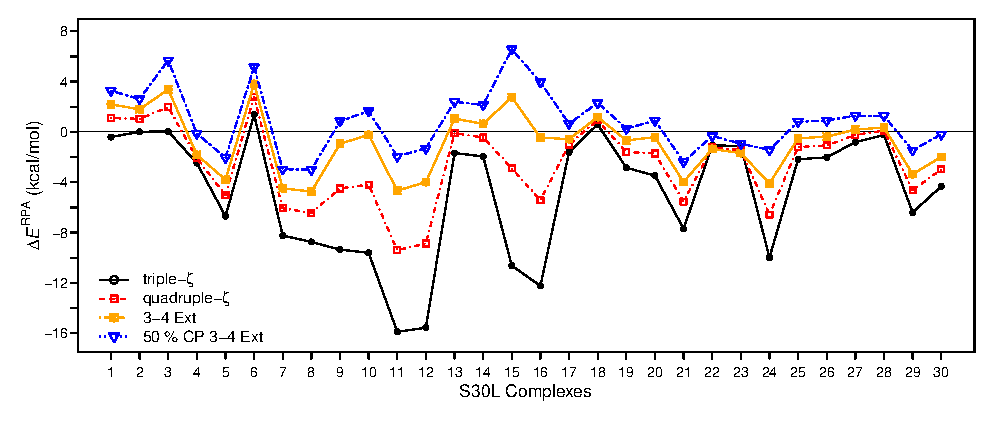
\includegraphics{conv_v5}
  \caption{S30L interaction energy errors ($\Delta E^{\text{RPA}}$)
    computed using RPA(PBE) with correlation-consistent triple-$\zeta$ and 
    quadruple-$\zeta$ basis sets, as well as using triple-quadruple (3-4)
    extrapolation with 50$\%$ and without counterpoise (CP) correction. DLPNO-CCSD(T)
    reference values are from Caldeweyher \textit{et al}.\cite{doi:10.1063/1.5090222}}
  \label{fig:conv}
\end{figure}

For the ROT34 benchmark,\cite{C3CP52293H,Risthaus14JComputChem35p1509} 
def2-QZVP basis sets were used for both the KS expectation value and
the RPA correlation; core electrons were treated explicitly. This approach
is expected to yield RPA structures of near basis-set limit quality
\cite{Burow14JChemTheoryComput10p180}. Indeed, changing
the basis sets from def2-TZVP 
to def2-QZVP only yields a small but systematic decrease in the error in
the RPA rotational constants, see Supporting Information.

\section{Results}
\label{sec:results}
\subsection{S66, L7, and S30L Interaction Energy Benchmarks}

\begin{table}[hbtp]
  \caption[hbtp]{Mean absolute errors (MAE), mean errors (ME),
    and absolute minimum-maximum error range (MinMax) in
    kcal/mol of 
    various methods at complete basis set 
    limit for the S66, L7, and S30L test sets. Positive ME corresponds
    to underbinding.}
  \label{tab:s30l}
  \resizebox{\textwidth}{!}{
  \begin{tabular}{cCCC@{\qquad}CCC@{\qquad}CCC@{\qquad}}
    \hline
    & \multicolumn{3}{c}{\text{S66}} & \multicolumn{3}{c}{\text{L7}} & \multicolumn{3}{c}{\text{S30L}}\\
    \cline{2-10}
    \text{Methods} & \text{MAE} & \text{ME~} & \text{MinMax~}
    & \text{MAE} & \text{ME~} & \text{MinMax~}
    & \text{MAE} & \text{ME~} & \text{MinMax~}\\
    \hline
    \text{RPA(PBE)}  & 0.61 & 0.61 & 1.00 & 1.72 & 1.47 & 3.53 & 2.03 & 0.82 & 6.44\\
    \text{RPA(TPSS)} & 0.63 & 0.63 & 1.02 & 1.92 & 1.73 & 3.75 & 2.05 & 1.33 & 8.64\\
    \text{MP2}
    & 0.35 &-0.54 & 2.30 & 8.77 &-8.77 & 17.51 & 18.74 &-18.74 & 66.07\\
    \text{MP3\textsuperscript{\emph{a}}}
    & 0.47 & 0.47 & 1.93 & 6.71 & 6.26 & 13.13 & -- & -- & --\\
    \text{SCS-MP2}
    & 0.32 & 0.64 & 1.92 & 2.49 & -1.41 & 5.77 & 7.43 &-4.68 & 33.47\\
    \text{SOS-MP2}
    & 0.65 & 1.23 & 2.57 & 2.28 & 2.27 & 5.83 & 6.26 & 2.35 & 16.26\\
    \text{PBE-D3\textsuperscript{\emph{b}}}
    & 0.34 &-0.24 & 1.93 & 1.91 & 0.92 & 4.39 & 3.06 & 1.83 & 9.80 \\
    \text{PBE-D4\textsuperscript{\emph{b}}}
    & 0.34 &-0.30 & 1.66 & 1.71 & 0.16 & 2.44 & 2.94 & -0.77 & 9.30\\
    \text{PW6B95-D3\textsuperscript{\emph{b}}}
    & -- & -- & -- & 1.39 & 1.19 & 2.20 & 1.82 & 0.32 & 4.70\\
    \text{PW6B95-D4\textsuperscript{\emph{b}}}
    & -- & -- & -- & 1.80 & 1.40 & 3.30 & 2.02 & 0.96 & 4.10\\
    \hline
  \end{tabular}}
  \begin{flushleft}
  \textsuperscript{\emph{a}} MP3 values from Refs.~\citenum{doi:10.1021/ct2002946}
  and \citenum{doi:10.1021/ct400036b}.
  
  \textsuperscript{\emph{b}} Dispersion corrected DFA values for L7 and S30L
  from Ref. \citenum{doi:10.1063/1.5090222}.
  \end{flushleft}
\end{table}

The S66 benchmark consists of binding energies of 66 complexes ranging
from 6 to 34 atoms; the average binding energy is 5.50 kcal/mol.
\cite{doi:10.1021/ct2002946,doi:10.1021/ct200523a}
This benchmark set is divided into groups featuring hydrogen bonding, $\pi$--$\pi$
stacking, aliphatic--aliphatic interactions,  $\pi$--aliphatic interactions,
and other nonspecific interactions, respectively. For the binding energies of
these complexes, 
MBPT is accurate: MP2 and third-order MP MBPT (MP3) yield mean absolute
errors (MAEs) of 0.35 kcal/mol and 0.47 kcal/mol, respectively. The
errors of dispersion-corrected DFT and MP2 variants are comparable. The
good performance of dispersion corrected DFAs is hardly surprising here
since S66 is part of commonly used training sets for parameter
estimation. \cite{Caldeweyher17JChemPhys147p034112}

The L7 benchmark contains binding energies of seven complexes: Octadecane
dimer, guanine trimer, circumcoronene--adenine dimer, coronene dimer,
guanine--cytosine dimer, circumcoronene--guanine--cytosine dimer, and an
amyloid fragment trimer containing 
phenylalanine residues; the average binding energy is 16.7
  kcal/mol.\cite{doi:10.1021/ct400036b,doi:10.1063/1.5012601} As shown in 
Table~\ref{tab:s30l}, 
MP2 performs poorly with an MAE of 8.10 kcal/mol, which is an order of
magnitude more larger for S66. Aside from the dependence of errors on
system size 
discussed in Section~\ref{subsub:size_dependence}, MP2 is known to
systematically overestimate $\pi$--$\pi$ stacking interactions even in
smaller systems.\cite{doi:10.1021/ct2002946} The inclusion of higher
orders does not systematically improve the MBPT results. For both, the S66 
and L7 benchmark sets, MP2 and MP3 mean errors are on the same orders of
magnitude but of opposite sign. Empirically, one observes that odd MBPT orders
tend to produce underbinding, whereas even orders produce
overbinding.\cite{doi:10.1021/jp952815d,doi:10.1063/1.481764}
The poor performance of MBPT for L7 and especially S30L is
in sharp contrast to the one observed for RPA, dispersion corrected PBE-D3,
and the recently developed PBE-D4,\cite{Caldeweyher17JChemPhys147p034112}
which all yield MAEs in the range of 2 kcal/mol. The RPA L7 results
reported here are $\sim 50$\% more accurate than the ones previously
obtained using def2-TZVP basis sets \cite{doi:10.1021/acs.jctc.6b01235},
underlining the importance of basis set extrapolation for RPA
interaction energy benchmarks \cite{Eshuis12JChemPhys136p084105}. 

\begin{figure}[hbpt]
  \centering
  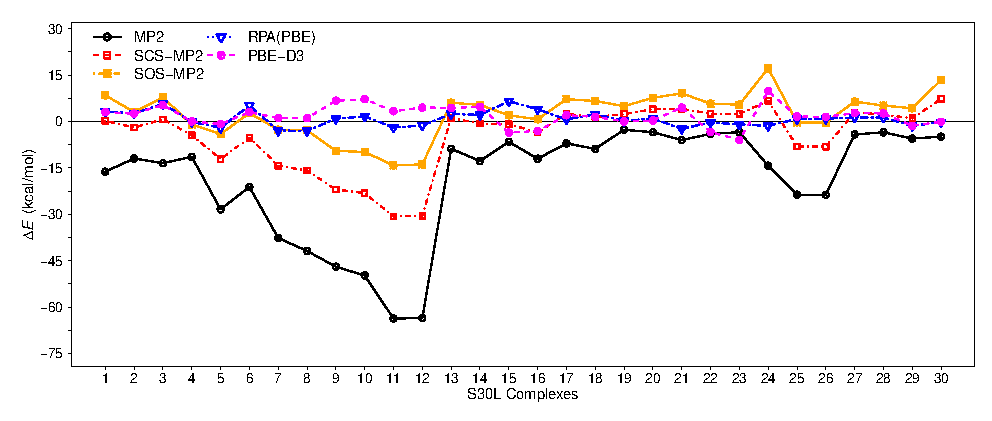
\includegraphics{s30l_compare2.eps}
  \caption{S30L interaction energy errors ($\Delta E$) for MP2 variants,
    RPA(PBE), and dispersion corrected PBE-D3. MP2 and RPA(PBE)
    results are 3-4 extrapolated, and PBE-D3 results use def2-QZVP basis
    sets. DLPNO-CCSD(T) reference values are from
    Caldeweyher \textit{et al}.\cite{doi:10.1063/1.5090222}}
  \label{fig:theories}
\end{figure}

The S30L benchmark set contains binding energies of 30 large supramolecular
complexes including $\pi$ stacking and CH--$\pi$ interactions, hydrogen
and halogen bonding, and charged 
species; the average binding energy is 37.5
  kcal/mol.\cite{Sure15JChemTheoryComput,doi:10.1063/1.5012601} MP2 exhibits severe
overbinding for most species, producing spectacular errors 
$>60$ kcal/mol for the $\pi$ stacked complexes 11 and 12, see Figure
\ref{fig:theories} and 
Table \ref{tab:s30l}. With MAEs of 7.43 and 6.26 kcal/mol, SCS-MP2 and
the SOS-MP2 inherit the shortcomings of MP2 to a significant degree.
RPA yields MAEs close to 2 kcal/mol regardless of the KS reference,
consistent with its performance observed for L7. Dispersion corrected
DFAs show comparable MAEs, but behave less systematically than RPA, as
evidenced by somewhat larger absolute minimum-maximum error ranges. The
present S30L results for RPA are more than twice as accurate as the ones
reported by He{\ss}elmann for the S12L subset \cite{heelmann201765};
this is likely a consequence of the improved CCSD(T) reference values 
\cite{doi:10.1063/1.5090222} used here as well as better controlled basis set
errors.

\subsection{ROT34: Intramolecular Interactions}

To investigate whether the strong performance of RPA for intermolecular
binding energies translates to other properties such as molecular
structures of larger flexible molecules, the equilibrium structures of 
34 organic molecules contained in the ROT34 benchmark\cite{C3CP52293H,Risthaus14JComputChem35p1509}
were optimized using RPA with def2-QZVP basis sets;
rotational constants
were calculated in the rigid rotor approximation. Rotational constants
are a sensitive measure of intramolecular mid- and long-range
interactions, and accurate experimental values are available from
gas-phase rotational spectroscopy. \cite{C3CP52293H,Risthaus14JComputChem35p1509}

As displayed in Figure~\ref{fig:methods_bar},
the PBE DFA produces a MAE of 18.2 MHz, even with D3 dispersion correction;
the Minnesota DFA M06L\cite{doi:10.1063/1.2370993}
and the strongly constrained and appropriately normed (SCAN)\cite{PhysRevLett.115.036402}
DFA perform significantly better:\cite{BrandenburgPhysRevB} For SCAN, SCAN-D3,
and M06L MAEs of 3.7 MHz, 3.3 MHz, and 4.0 MHz were
reported.\cite{BrandenburgPhysRevB} The MAEs of MP2 
and SCS-MP2, on the other hand, are 5.5 MHz and 5.4
MHz,\cite{Risthaus14JComputChem35p1509} respectively, comparing
unfavorably with the RPA(PBE) result of 3.1 MHz; using the TPSS instead
of the PBE DFA to generate the KS reference yields an almost identical
MAE of 3.0 MHz. Thus, even for the moderately sized systems contained in
ROT34, the sub-par performance of MP2 is notable.

\begin{figure}[hbtp]
   \centering
  \includegraphics{deviate_v4.eps}
  \caption{Errors in ROT34 computed rotational constants compared to
    experiment.\cite{Risthaus14JComputChem35p1509}  
    Mean absolute errors (MAE) and mean errors (ME) are in MHz,
    and relative minimum-maximum error ranges
    (rMinMax) are in $\%$. MP2 and SCS-MP2 results are from
    Ref. \citenum{Risthaus14JComputChem35p1509}; and SCAN, SCAN-D3,
    PBE-D3, and M06L results are from Ref. \citenum{BrandenburgPhysRevB}.}
  \label{fig:methods_bar}
\end{figure}

\section{AC-SAPT Analysis}
\label{sec:SAPT}

\subsection{Statement of the Problem}

In the following, the results of the previous sections are analyzed in
two steps: First, we derive asymptotically exact expressions for the
dispersion energy at large separation. We rely on the general SAPT
partitioning of the Hamiltonian \cite{doi:10.1063/1.461528}, but unlike
prior DFT-SAPT  methods\cite{doi:10.1002/wcms.1164,PhysRevLett.91.033201} 
or van-der-Waals inclusive frozen density embedding,\cite{doi:10.1021/j100132a040, 
  doi:10.1063/1.4890839} 
the present AC-SAPT approach uses density functional theory only for the
inter-fragment interaction and constrains the density of the monomers,
leading to compact closed-form expressions for the interaction energy
and a separation of dispersion and induction effects. We derive an upper
bound for the convergence radius of the resulting AC-SAPT expansion. Second,
we show that the RPA dispersion energy corresponds to a partial resummation
of the AC-SAPT expansion, whereas the MBPT dispersion energy corresponds to a
finite-order approximation. When the monomers are treated within RPA,
the AC-SAPT converges for nondegenerate monomers, whereas it is found to be
susceptible to spurious divergence for MBPT treatments of the monomers.

We consider a molecular supersystem or complex A--B consisting of two
non-overlapping subsystems or fragments A and B, i.e., the  
inter-fragment distance $R$ is assumed to be so large 
that the overlap between the two ground states is exponentially
small. Since there is vanishing charge transfer in this limit, the
fragments have integer electron numbers $N_\text{A}, N_\text{B}$ with
ground states 
resembling the lowest-energy separated fragment (dissociation) limit of A--B.
The Born--Oppenheimer Hamiltonian of the supersystem at coupling strength
$\alpha$ is
\begin{equation}
  \hat{H}^\alpha = \hat{H}_{\text{A}} + \hat{H}_{\text{B}} + \alpha
   \hat{V}_{ee \,\text{int}}  + \hat{V}_{s\,\text{int}}^\alpha[\rho] ,
\end{equation}
where $\hat{H}_{\text{A}}$ and $\hat{H}_{\text{B}}$ denote the
$N_\text{A}$- and $N_\text{B}$-electron Hamiltonians of the isolated
subsystems, and
$\hat{V}_{ee \,\text{int}}$ is the operator of the electron-electron
Coulomb interaction \emph{between} A and
B. The supersystem eigenstates $\ket{\Psi_n^\alpha}$, which are
constrained to be
antisymmetric under any permutations of electrons in the supersystem as
in conventional SAPT,
and their energies $E^\alpha_n$ are defined by
\begin{equation}
  \hat{H}^\alpha \ket{\Psi_n^\alpha} = E^\alpha_n
  \ket{\Psi_n^\alpha}.
\end{equation}
$\hat{V}_{s\,\text{int}}^\alpha[\rho]$ represents a   
local one-electron potential which constrains the density of the 
supersystem ground state $\ket{\Psi^\alpha_0}$ to the physical ground-state
density $\rho = \rho^1 = \left.\rho^\alpha\right|_{\alpha=1}$. Since
$\hat{V}_{s\,\text{int}}^\alpha[\rho]$ is a unique
functional of $\rho$,\cite{PhysRev.136.B864} so are $\ket{\Psi^\alpha_n}$
and the corresponding energies $E^\alpha_n$. Throughout this paper, the
ground state $\ket{\Psi^\alpha_0}$ is assumed to be nondegenerate for
finite $R$, a mild condition typically satisfied for interacting
closed-shell fragments. The use of symmetry adaption implies that the
present approach is valid only at large $R$ as in conventional SAPT,
\cite{doi:10.1063/1.463475} but
this is sufficient for asymptotic analysis.

In analogy with the conventional KS potential,
  \begin{equation}
    \label{eq:vsdef}
    \hat{V}_{s\,\text{int}}^\alpha[\rho] =  \hat{V}_{ne
        \,\text{int}} + V_{nn \,\text{int}} +
    \hat{V}_{\text{int}}^{\text{HXC}}[\rho] -
    \hat{V}_{\text{int}}^{\alpha\text{HXC}}[\rho]
  \end{equation}
may be defined as a sum of the ``external'' one-electron
nucleus-electron potential $\hat{V}_{ne\,\text{int}}$ and the constant
nucleus-nucleus attraction $V_{nn \,\text{int}}$ between the fragments
plus a remainder accounting for Hartree-, exchange-, and correlation
(HXC) effects. At full coupling ($\alpha=1$), the HXC part of
$\hat{V}_{s\,\text{int}}^\alpha[\rho]$ vanishes, whereas at $\alpha=0$,
$\hat{V}_{s\,\text{int}}^\alpha[\rho]$ equals  
the KS potential arising from the interaction between the
fragments. Since the KS 
potential is spatially local, it additively separates into A and B parts for
large $R$, giving rise to a unique partitioning of the supersystem
density into a sum of
subsystem densities, i.e., $\rho(x) = \rho_{\text{A}}(x)+\rho_{\text{B}}(x)$. 
Thus, the present approach is closely related to
partition DFT (PDFT).\cite{Cohen2006,PhysRevA.82.024501} However,
PDFTs\cite{doi:10.1002/wcms.1164,PhysRevLett.91.033201} and related embedding
schemes\cite{doi:10.1021/j100132a040,doi:10.1063/1.4890839}
typically start from a KS-DFT calculation of the supersystem, whereas here the
fragment ground states corresponding to $\alpha=0$ include the full
intra-fragment electron-electron interaction and therefore are
generally not Slater determinants.

\subsection{Interaction Energy}

We define the A--B interaction energy as the difference in the ground
state energies at full and zero coupling,
\begin{equation}
  % E_{\text{int}}[\rho] =
  % E^\alpha[\rho]|_{\alpha=1}-E^\alpha[\rho]|_{\alpha=0}
  E_{\text{int}}[\rho] =
  E^1_0[\rho] - E^0_0[\rho].
\end{equation}
Using the Hellman--Feynman theorem, the interaction energy may be
expressed as a coupling strength 
average of the potential energy of interaction\cite{PhysRevA.82.024501},
\begin{equation}
  E_{\text{int}}[\rho] = \int_0^1 d\alpha\, W^\alpha[\rho],
\end{equation}
where $W^\alpha[\rho] = dE_0^{\alpha}/d\alpha = \braket{ \Psi^\alpha_0 |
    \hat{V}_{ee \,\text{int}} | \Psi^\alpha_0 }$;
one-electron contributions vanish upon coupling strength integration due
to the density constraint. The AC-SAPT expansion of the interaction
energy is obtained by expansion of the interacting ground state
and the corresponding energy into powers of $\alpha$, analogous to
G{\"o}rling--Levy perturbation theory.\cite{PhysRevB.47.13105,PhysRevA.52.4493}
Equivalently, the coupling strength integrand $W^\alpha$ may be expanded around
$\alpha=0$, yielding the AC-SAPT series expansion of the interaction
energy, 
\begin{equation}
  \label{eq:acsapt}
  E_{\text{int}}[\rho] = \int_0^1 d\alpha \sum_{k = 0}^{\infty} \alpha^k
  W^{(k)}[\rho] = \sum_{k=0}^{\infty} \frac{1}{k+1} W^{(k)}[\rho].
\end{equation}

The first-order interaction energy results from evaluating the integrand
at $\alpha=0$, 
\begin{equation}
  E_{\text{int}}^{(1)}[\rho] = \braket{ \Psi^0_0 |
    \hat{V}_{ee \,\text{int}} | \Psi^0_0 } = E^{\text{HX}}_{\text{int}}[\rho] = 
  \int dx_1 dx_2 \frac{ \rho_A(x_1)
    \rho_B(x_2) - \gamma_A(x_1,x_2)\gamma_B(x_2,x_1) }{|\mathbf{r}_1-\mathbf{r}_2|},
\end{equation}
where $\ket{\Psi^0_0}$ is the antisymmetrized
product of the two fragment density-constrained ground-state
wavefunctions with one-particle 
density matrices $\gamma_A, \gamma_B$. As in standard SAPT, the
first-order interaction 
energy is electrostatic and corresponds to the sum of the Hartree
and exchange (HX) interactions between the two fragments; unlike in standard
SAPT, and as discussed in detail below, the interaction arises from the
electrons only. The exchange term 
is exponentially small for non-degenerate ground states in the large $R$
limit. 

The remaining correlation part of the interaction energy,
\begin{equation}
  \label{eq:ecint}
  E^{\text{C}}_{\text{int}}[\rho] = \int_0^1 d\alpha \left( \braket{ \Psi^\alpha_0 |
    \hat{V}_{ee \,\text{int}} | \Psi^\alpha_0 } - \braket{ \Psi^0_0 |
    \hat{V}_{ee \,\text{int}} | \Psi^0_0 } \right)  
\end{equation}
is due to dispersion and does not contain any terms describing changes
in the fragment densities as the interaction is turned on. 
The purely dispersive character of the interaction becomes apparent from
a factorization of $\hat{V}_{ee \,\text{int}}$ 
in a fashion analogous to Eqs. (6)-(13) of
Ref. \citenum{Eshuis12TheorChemAcc131p1084} and neglecting exponentially
small exchange terms, yielding
\begin{equation}
  \label{eq:fdisp}
  E^{\text{C}}_{\text{int}}[\rho] = \int_0^1 d\alpha \int dx_1 dx_2
  \frac{ \braket{ \Psi^\alpha_0 | \Delta \hat{\rho}_A(x_1) \Delta
      \hat{\rho}_B(x_2) | \Psi^\alpha_0 } - \braket{ \Psi^0_0 |
      \Delta \hat{\rho}_A(x_1) \Delta 
      \hat{\rho}_B(x_2) | \Psi^0_0 }  }{|\mathbf{r}_1-\mathbf{r}_2|},
\end{equation}
where $\Delta \hat{\rho}_A(x) = \hat{\rho}_A(x) - \rho_A(x)$ is the
density fluctuation operator associated with fragment A,
$\hat{\rho}_A(x)$ is the corresponding density operator, and $\Delta
\hat{\rho}_B(x)$ is defined analogously. 
As opposed to standard SAPT (including DFT-SAPT), which is based on a
partitioning of the Hamiltonian that includes induction effects to all
orders, the interaction energy in the present approach 
does not contain any
induction terms and is exclusively due to electrostatic (Hartree plus
exchange) and dispersion. Factorization of the density operator product in
Eq.~\eqref{eq:fdisp} using the completeness of the eigenstates of
$\hat{H}^\alpha$ yields a spectral sum over Hartree
interactions between the A and B parts of  ground-to-$n$-th excited
state transition densities $\rho_{0n}^\alpha(x) = \rho_{n0}^{\alpha *}(x)$, 
\begin{equation}
  \label{eq:edyn}
  E^{\text{C}}_{\text{int}}[\rho] = \sum_{n\ne 0} \int_0^1 d\alpha \int dx_1 dx_2
  \frac{ \rho^\alpha_{0n\,A}(x_1) \rho^\alpha_{n0\,B}(x_2)  -
    \rho^0_{0n\,A}(x_1) \rho^0_{n0\,B}(x_2)
  }{|\mathbf{r}_1-\mathbf{r}_2|}. 
\end{equation}
The $\alpha=0$ term vanishes for large $R$ since excitations of the
non-interacting monomers are localized on either monomer, but is
included here to emphasize the analogy to general RPA theory
\cite{Furche08JChemPhys129p114105}.
In this sense, the A--B dispersion energy is given exactly by the
Hartree interaction between ``electrodynamic'' density fluctuations of
the monomers. While similar ideas are implicit, e.g., in molecular
quantum electrodynamics,\cite{craig1998molecular}
the present approach yields a compact, exact expression valid beyond
perturbation theory. The induction energy, on the other hand, appears as
the difference between the non-interacting 
($\alpha =0$) monomer ground state energies with and without density
constraint,
\begin{equation}
  \label{eq:eind}
  E_{\text{ind}} = E^0[\rho] - E_{\text{A}} - E_{\text{B}}.
\end{equation}
The total dissociation energy of the complex A--B is thus
\begin{equation}
  \label{eq:etot}
  D_{\text{A--B}} = E_{\text{int}}[\rho] + E_{\text{ind}}.
\end{equation}
Induction effects are comparatively small for large $R$;\cite{doi:10.1002/wcms.86}
hence, we will focus on $E_{\text{int}}[\rho]$ in the following.

If the zero-point fluctuation--dissipation theorem (FDT) is invoked
\cite{Langreth77PhysRevB15p2884,Langreth75SolidStateCommun17p1425, 
  PhysRevB.13.4274,PhysRevB.15.6006.3,Dobson12JPhysCondensMatter24p073201}
to factorize the products of fluctuation operators in
Eq. \eqref{eq:fdisp}, the dispersion energy may be expressed as 
\begin{equation}
  \label{eq:fdt}
  E_{\text{int}}^{\text{C}}[\rho] = -\frac{1}{2} \int_0^1 d\alpha
  \int_{-\infty}^{\infty} \frac{dz}{2\pi i} 
  \left\langle
  \left(
    \boldsymbol{\Pi}^\alpha(z) - \boldsymbol{\Pi}^0(z)
  \right) 
  \mathbf{V}_{\text{int}}
  \right\rangle.
\end{equation}
Here, $\boldsymbol{\Pi}^\alpha(z)$ is the time-ordered supersystem
polarization propagator at coupling strength
$\alpha$ and imaginary frequency $z=i\omega \in i \mathbf{R}$ defined as
\cite{fetter_walecka_1971}   
\begin{equation}
  \label{eq:pidef}
  \boldsymbol{\Pi}^\alpha(z) = - \sum_{n \ne 0} \left\{
    \frac{ \boldsymbol{\gamma}_{0n}^\alpha \otimes
      \boldsymbol{\gamma}_{0n}^{\alpha \dag}} {z -
      \Omega_n^\alpha + i 0^+ } - \frac{
      \boldsymbol{\gamma}_{0n}^{\alpha \dag} \otimes 
      \boldsymbol{\gamma}_{0n}^\alpha } { z +
      \Omega_n^\alpha - i 0^+ } \right\}.
\end{equation}
$\Omega_n^\alpha = E_n^\alpha-E_0^\alpha$ is the
energy of an excitation from $\ket{\Psi^\alpha_0}$ to
$\ket{\Psi^\alpha_n}$, and $\boldsymbol{\gamma}_{0n}^\alpha$
denotes the corresponding one-particle transition density
matrix. 
Eq.~\eqref{eq:pidef} shows that, for non-degenerate monomer ground states,
$\boldsymbol{\Pi}^\alpha(z)$ 
is a self-adjoint and negative semidefinite operator on the
tensor-product space of one-particle operators.  
$\mathbf{V}_{\text{int}}$ represents the bare inter-fragment
electron-electron Coulomb interaction or the Hartree kernel on the same
space. 

Eqs.~\eqref{eq:fdisp}-\eqref{eq:edyn} could
also be
used to define the dispersion energy in conjunction with
MP-style partitioning of the Hamiltonian, using the
analogous, albeit approximate, HF-based AC
framework \cite{Eshuis12TheorChemAcc131p1084}. Formally, this
corresponds to replacing the local exchange-correlation potential in
Eq.~\eqref{eq:vsdef} with the non-local HF exchange potential. The
$\alpha=0$ reference of this
approach is equivalent to monomers with full intra-fragment
electron-electron interaction whose inter-fragment interaction is
treated at the Hartree plus exchange level. In the HF-based AC framework, the
interaction energy obtained from coupling strength integration contains
additional induction effects resulting from changes in the fragment densities
due to inter-fragment correlation which are not captured by the
FDT, but the present conclusions for the
dispersive part of the interaction energy remain valid.

\subsection{Dispersion Energy}

Expression \eqref{eq:fdt} for the dispersion energy can be further
re-cast by noting that any contributions from
charge transfer excitations between the fragments vanish exponentially
due to exponentially vanishing overlap at large $R$; it therefore
suffices to consider $\boldsymbol{\Pi}^\alpha(z)$ on the domain of
fragment-centered excitations only.
Thus,
$\boldsymbol{\Pi}^\alpha(z)$ may be partitioned as 
\begin{equation}
    \boldsymbol{\Pi}^\alpha(z) = 
    \begin{pmatrix}
    \boldsymbol{\Pi}^\alpha_\text{AA}(z) & \boldsymbol{\Pi}^\alpha_\text{AB}(z) \\
    \boldsymbol{\Pi}^\alpha_\text{BA}(z) & \boldsymbol{\Pi}^\alpha_\text{BB}(z) 
    \end{pmatrix},
  \end{equation}
where indices AA refer to the 4-index tensor space spanned by products
of transition density matrices centered on fragment A, etc. In the
non-interacting ($\alpha=0$) case, all excitations are either
excitations of A or B only, hence
$\boldsymbol{\Pi}^0_\text{AB}(z) =
\boldsymbol{\Pi}^0_\text{BA}(z) = \mathbf{0}$, and the diagonal
parts reduce to the fragment polarization propagators (at full
intra-fragment coupling).
The inter-fragment Coulomb interaction may be partitioned as
\begin{equation}
  \mathbf{V}_{\text{int}} = \begin{pmatrix}
    \mathbf{0} & \mathbf{V}_{\text{AB}}\\
     \mathbf{V}_{\text{BA}} & \mathbf{0} \end{pmatrix},
\end{equation}
where the diagonal blocks must vanish to recover the correct monomer
limit at large $R$.

It is instructive to introduce the dielectric operator
$\boldsymbol{\epsilon}^\alpha(z)$ (also called generalized dielectric
function or matrix\cite{PhysRevB.47.9892,PhysRevX.6.041002}) via
\begin{equation}
  \label{eq:epsdef}
  \boldsymbol{\Pi}^\alpha(z) =
  \boldsymbol{\epsilon}^\alpha(z)^{-1} \boldsymbol{\Pi}^0(z).
\end{equation}

In the spirit of the Bethe--Salpeter equation,\cite{fetter_walecka_1971}
$\boldsymbol{\epsilon}^\alpha(z)$ 
may be expressed as
\begin{equation}
    \boldsymbol{\epsilon}^\alpha(z) = \mathbf{1} -
    \boldsymbol{\Pi}^0(z) \mathbf{K}^{\alpha\text{HXC}}_{\text{int}}(z),
\end{equation}
where
$\mathbf{K}^{\alpha\text{HXC}}_\text{int}(z)$ denotes the 
imaginary-frequency-dependent HXC kernel at coupling strength $\alpha$
for the intersystem interaction. 
Similar to the Hartree kernel, the elements in the diagonal blocks of
$\mathbf{K}^{\alpha\text{HXC}}_\text{int}(z)$ vanish, because
$\boldsymbol{\Pi}^0(z)$ contains the full intra-fragment
interaction.

Since $\mathbf{V}_{\text{int}}$ and $\mathbf{K}^{\alpha\text{HXC}}_\text{int}$
have vanishing diagonal blocks, these can be used to further simplify the  
dispersion energy: Noting that the diagonal blocks of $\boldsymbol{\Pi}^0(z)
\mathbf{V}_{\text{int}}$ vanish, and using
Eq.~\eqref{eq:epsdef}, the FDT \eqref{eq:fdt} takes the form
\begin{equation}
  \label{eq:fdts}
  E_{\text{int}}^{\text{C}}[\rho] = -\frac{1}{2} \int_0^1 d\alpha
  \int_{-\infty}^{\infty} \frac{dz}{2\pi i} \left\langle
      \boldsymbol{\epsilon}^\alpha(z)^{-1} \boldsymbol{\Pi}^0(z)
    \mathbf{V}_{\text{int}} \right\rangle.
\end{equation}
For similar reasons, all even orders in the geometric series expansion of
$ \boldsymbol{\epsilon}^\alpha(z)^{-1}$ with respect to
$\boldsymbol{\Pi}^0(z)
\mathbf{K}^{\alpha\text{HXC}}_{\text{int}}(z)$ do not contribute
to the dispersion energy. It is hence convenient to define the second-order  
generalized dielectric function 
\begin{equation}
  \label{eq:kappadef}
  \boldsymbol{\kappa}^\alpha(z) = \boldsymbol{\epsilon}^\alpha(z) \left(
  \mathbf{2} - \boldsymbol{\epsilon}^\alpha(z) \right) =  \mathbf{1} -
  \left( \boldsymbol{\Pi}^0(z) 
  \mathbf{K}^{\alpha\text{HXC}}_\text{int}(z) \right)^2,
\end{equation}
which is block diagonal with exponentially vanishing off-diagonal blocks. 
Substituting Eq.~\eqref{eq:kappadef} into Eq.~\eqref{eq:fdts} and using
the vanishing trace of 
$\boldsymbol{\kappa}^\alpha(z)^{-1}\boldsymbol{\Pi}^0(z)
\mathbf{V}_\text{int}$, we arrive at a central theoretical 
result of this paper, 
\begin{equation}
  \label{eq:ecabfin}
  E_{\text{int}}^{\text{C}}[\rho] = -\frac{1}{2} \int_0^1 d\alpha
  \int_{-\infty}^{\infty} \frac{dz}{2\pi i} \left\langle
    \boldsymbol{\kappa}^\alpha(z)^{-1} 
    \boldsymbol{\Pi}^0(z)
    \mathbf{K}^{\alpha\text{HXC}}_\text{int}(z) 
    \boldsymbol{\Pi}^0(z) \mathbf{V}_{\text{int}}
 \right\rangle. 
\end{equation}

Eq.~\eqref{eq:ecabfin} ``exactifies'' the well-known
Longuet-Higgins Zaremba-Kohn\cite{df9654000007,PhysRevB.13.2270}
expression for the second-order dispersion energy, denoted LHZK(2)
in the following. Eq.~\eqref{eq:ecabfin} goes beyond LHZK(2) by
including (i) exchange and correlation effects in the AB interaction through
$\mathbf{K}^{\alpha\text{HXC}}_\text{int}$, and (ii) screening 
of the bare Coulomb interaction $\mathbf{V}_{\text{int}}$ by
$\boldsymbol{\kappa}^\alpha(i\omega)$. Indeed, the
replacements $\mathbf{K}^{\alpha\text{HXC}}_\text{int} \rightarrow \alpha
\mathbf{V}_{\text{int}}$ and $\boldsymbol{\kappa}^\alpha(z)
\rightarrow \mathbf{1}$ recover LHZK(2). Figure \ref{fig:goldstone}
displays a diagrammatic representation
of
Eq.~\eqref{eq:ecabfin}.

\begin{figure}[hbtp]
  \centering
  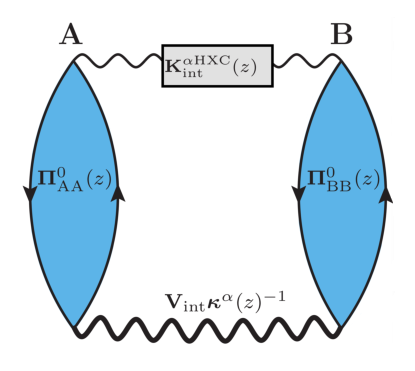
\includegraphics[width=0.5\linewidth]{int_gold.eps}
  \caption{Diagrammatic representation of the A--B dispersion energy
    Eq. \eqref{eq:ecabfin}. Blue-shaded rings with upward--downward
    arrows denote particle--hole propagators of the monomers containing
    the full intra-monomer interaction, whereas horizontal wavy lines
    represent interactions between the monomers. Coupling strength and
    frequency integration are implied.}
  \label{fig:goldstone}
\end{figure}

\subsection{Convergence Radius of the AC-SAPT Series}

The convergence of the AC-SAPT series, Eq.~\eqref{eq:acsapt}, is governed by
the analyticity of the coupling strength 
integrand $W^\alpha[\rho]$ in the complex $\alpha$ plane: To
guarantee convergence, the 
coupling strength integrand must be analytic for $|\alpha| \le
1$. Using Eq.~\eqref{eq:fdts}, this implies that
$\boldsymbol{\epsilon}^\alpha(z)^{-1}$ must give rise to an analytic
coupling strength integrand for $|\alpha| \le
1$. A necessary condition for the latter is that
$\boldsymbol{\epsilon}^\alpha(z)^{-1}$ is free of poles, i.e., by
Eq.~\eqref{eq:epsdef},
\begin{equation}
  \label{eq:conv}
  \left\| \boldsymbol{\Pi}^0(z) \mathbf{K}^{\alpha\text{HXC}}_\text{int}(z)
    \right\|_2 = \left\| \mathbf{1} -
    \boldsymbol{\epsilon}^\alpha(z) \right\|_2 < 1. 
\end{equation}
Here, the spectral norm $\|\cdot\|_2$ equals the largest singular value
of an operator; $\|\cdot\|_2$ is induced by the scalar product on the
tensor product space and thus a natural choice. An upper bound for the
convergence radius of the AC-SAPT series is thus
\begin{equation}
  \label{eq:alphac}
  \alpha_c = \min_{\alpha}\left\{ |\alpha| : \left\| 
        \boldsymbol{\Pi}^0(z)
        \mathbf{K}^{\alpha\text{HXC}}_\text{int}(z) 
    \right\|_2 = 1
    \right\}.
\end{equation}
$\alpha_c$ is generally an upper bound for the convergence radius, since
$\boldsymbol{\epsilon}^\alpha(z)^{-1}$ could exhibit additional,
non-algebraic singularities inside the complex $\alpha$ unit
circle.

The convergence criterion \eqref{eq:conv} also implies that the
geometric series 
\begin{equation}
  \label{eq:giptgen}
  \boldsymbol{\kappa}^\alpha(z)^{-1} = \mathbf{1} +
  \left(\boldsymbol{\Pi}^0(z)
  \mathbf{K}^{\alpha\text{HXC}}_\text{int}(z) \right)^2 +
  \left(\boldsymbol{\Pi}^0(z)
  \mathbf{K}^{\alpha\text{HXC}}_\text{int}(z) \right)^4 + \ldots
\end{equation}
converges, since, by the definition of the spectral norm and the
negative definiteness of $\boldsymbol{\Pi}^0(z)$,
\begin{equation}
  \label{eq:convgen}
  \left\| \mathbf{1} -
    \boldsymbol{\kappa}^\alpha(z) \right\|_2 = \left\| \left(
      \boldsymbol{\Pi}^0(z) \mathbf{K}^{\alpha\text{HXC}}_\text{int}(z)
    \right)^2 \right\|_2 =  \left\| 
      \boldsymbol{\Pi}^0(z) \mathbf{K}^{\alpha\text{HXC}}_\text{int}(z)
     \right\|_2^2 < 1. 
\end{equation}
Necessary conditions equivalent to Eq. \eqref{eq:conv} are thus that
$\boldsymbol{\kappa}^\alpha(z)$ be positive definite or 
$\boldsymbol{\epsilon}^\alpha(z)^{-1}$ have eigenvalues $<2$.

\subsection{Approximations within AC-SAPT}

In the following, we determine the asymptotic expressions for the
dispersion energy corresponding to supermolecular RPA and MBPT
calculations, and analyze the consequences for the AC-SAPT expansion.

\subsubsection{Random Phase Approximation}
\label{sec:rpa}

The RPA polarization propagator
at zero intermonomer interaction,
\begin{equation}
  \label{eq:pirpa}
  \boldsymbol{\Pi}^\text{RPA}(z) = \left( \mathbf{1}-
    \boldsymbol{\Pi}^0_0(z) \mathbf{V}_0 \right)^{-1}
  \boldsymbol{\Pi}^0_0(z),
\end{equation}
is defined in terms of the bare KS 
polarization propagator of the supersystem $\boldsymbol{\Pi}^0_0$,
which does not include any electron-electron interactions, and the 
intramonomer interaction $\mathbf{V}_0$ with the matrix
representation
\begin{equation}
  \mathbf{V}_0 = \begin{pmatrix}
    \mathbf{V}_{AA} & \mathbf{0}\\
     \mathbf{0} & \mathbf{V}_{BB} \end{pmatrix}
\end{equation}
in the large $R$ limit. A supermolecular RPA calculation corresponds to the
replacements
\begin{equation}
  \label{eq:rparep}
\mathbf{K}^{\alpha\text{HXC}}_\text{int}(z)
\rightarrow \alpha \mathbf{V}_{\text{int}}\quad \text{and} \quad
\boldsymbol{\Pi}^0(z) 
\rightarrow \boldsymbol{\Pi}^\text{RPA}(z)
\end{equation}
in Eqs.~\eqref{eq:fdt}-\eqref{eq:alphac}. In other words, the
intramolecular electron correlation and the screening factor
$\boldsymbol{\kappa}^\alpha(z)^{-1}$ in Eq. \eqref{eq:ecabfin} are
treated non-perturbatively, whereas the intermolecular HXC kernel is
replaced by its first-order approximation.

Condition~\eqref{eq:conv} implies that, within RPA, the AC-SAPT series will
converge if 
\begin{equation}
  |\alpha| \left \| \boldsymbol{\Pi}^\text{RPA}(z)
    \mathbf{V}_{\text{int}} \right\|_2 < 1.
\end{equation}
This condition is necessary and sufficient for RPA, because the only
singularities of the RPA coupling strength integrand in the complex
$\alpha$ plane result from zeros of
\begin{equation}
  \label{eq:kapparpa}
  \boldsymbol{\kappa}^{\alpha\text{RPA}}(z) = \mathbf{1} - \alpha^2
  \left( \boldsymbol{\Pi}^{\text{RPA}}(z)
    \mathbf{V}_{\text{int}}\right)^2.
\end{equation}
The convergence radius thus has the lower bound
\begin{equation}
  \alpha_c^{\text{RPA}} = 
    \left \| \boldsymbol{\Pi}^\text{RPA}(z)
    \mathbf{V}_{\text{int}} \right\|_2^{-1} \geq \left\|
    \boldsymbol{\Pi}^\text{RPA}(z) \mathbf{V}_0 \right\|_2^{-1} 
    \left\|
    \mathbf{V}_0^{-1} \mathbf{V}_\text{int}
    \right\|_2^{-1}, 
\end{equation}
where the inequality follows from the submultiplicativity of the spectral norm.
Since $\boldsymbol{\Pi}^0(z)\mathbf{V}_0$ is negative
definite,
\begin{equation}
  \label{eq:rpabound}
  \left\| 
  \boldsymbol{\Pi}^\text{RPA}(z) \mathbf{V}_0 \right\|_2\leq 1
\end{equation}
by Eq.~\eqref{eq:pirpa}. Moreover, 
$\left\| \mathbf{V}_0^{-1} \mathbf{V}_\text{int}
\right\|_2 \leq 1$ follows \cite{horn199063} from the fact that both
$\mathbf{V}_0$ and $\mathbf{V}_0+\mathbf{V}_{\text{int}}$,
corresponding to the monomer-only and supersystem Hartree kernels, are
positive definite.
Consequently,
\begin{equation}
  \label{eq:alphacrpa}
  \alpha_c^{\text{RPA}} \ge 1,
\end{equation}
where the inequality holds as long as $\left\| 
\boldsymbol{\Pi}^0_0(z) \mathbf{V}_0 \right\|_2 <
\infty$. This condition is satisfied for monomers with finite KS gap,
where $ \boldsymbol{\Pi}^0_0(z)$ is bounded, 
but may be violated, e.g., for infinite one-dimensional metals, see below. 
Hence, the AC-SAPT series always converges within RPA for nondegenerate 
monomers.

RPA permits analytic integration over coupling strength in
Eq. \eqref{eq:ecabfin}, yielding a compact expression for the dispersion
energy within RPA,
\begin{equation}
  \label{eq:ecabrpa}
  E^{\text{C\, RPA}}_{\text{int}}[\rho] = \frac{1}{4}
  \int_{-\infty}^{\infty} \frac{d\omega}{2\pi} \langle \ln
    \boldsymbol{\kappa}^{\text{RPA}}(z) \rangle.
\end{equation}
Eq. \eqref{eq:ecabrpa} illustrates how the analytic
structure of $\ln \boldsymbol{\kappa}^{\text{RPA}}(z)$ governs the
convergence of the AC-SAPT expansion at full coupling within
RPA. For nondegenerate monomers, $\boldsymbol{\kappa}^{\text{RPA}}(z)$ is
positive definite with eigenvalues between 0 and 1, and thus the Taylor
expansion around $\boldsymbol{\kappa}^{\text{RPA}}(z) = \mathbf{1}$,
which generates the AC-SAPT series, converges. However, if
$\boldsymbol{\kappa}^{\text{RPA}}(z)$ has 
zero eigenvalues, the series diverges due to the essential
singularity of the natural logarithm at zero.

Dobson and Gould (DG) obtained Eq. \eqref{eq:ecabrpa} by a coupling strength
integration argument without density constraint, and showed that 
it reduces to the non-retarded Lifshitz formula for macroscopic slab
systems, which is accurate for dispersion interactions between macroscopic
objects.\cite{Dobson12JPhysCondensMatter24p073201} DG also identified 
conditions for which Eq. \eqref{eq:ecabrpa} predicts unconventional 
power laws of dispersion interactions that cannot be obtained from
AC-SAPT: Systems must be macroscopic in at least one dimension, allowing
for infinite-wavelength density fluctuations, finite in at least one
other dimension, and exhibit zero electronic gap. This is precisely when
$\boldsymbol{\kappa}^{\text{RPA}}(z)$ can have zero eigenvalues, causing
AC-SAPT to diverge. The unconventional power
laws observed \cite{PhysRevLett.96.073201} for these systems cannot be
obtained from a Taylor series with respect to $\alpha$ and thus are
examples of physical systems exhibiting divergence of AC-SAPT. 

\subsubsection{Many-Body Perturbation Theory}

In the present framework, supersystem MBPT calculations correspond to
perturbatively expanding the coupling strength integrand
$W^\alpha[\rho]$ with respect to 
both, the inter- and intramonomer interaction, such that the resulting
total interaction energy is consistent to a given finite
order. In the following, we consider supersystem MBPT(2) theory,
which is by far the most commonly used MBPT approach for NIs in large
molecular systems. Supersystem MBPT(2) corresponds to the replacements
\begin{equation}
  \label{eq:pt2ep}
\mathbf{K}^{\alpha\text{HXC}}_\text{int}(z)
\rightarrow \alpha \mathbf{V}_{\text{int}}\quad \text{and} \quad
\boldsymbol{\Pi}^0(z) 
\rightarrow \boldsymbol{\Pi}^0_0(z) \quad \text{and} \quad
\boldsymbol{\kappa}_{\alpha}(z) \rightarrow \mathbf{1}
\end{equation}
in Eqs. \eqref{eq:fdt}-\eqref{eq:alphac}. These replacements are
sufficient to make the coupling strength integrand correct to first
order, corresponding to MBPT(2) for the (coupling strength integrated)
correlation energy. In the present constant-density AC approach, this
is equivalent to second-order G{\"o}rling--Levy perturbation theory treatment
of the supersystem; analogous considerations apply to MP2. The replacements
\eqref{eq:pt2ep} amount to the LHZK(2) limit. This implies that the
geometric series \eqref{eq:giptgen} is truncated after the first term, which
is likely to result in large errors unless the series converges very rapidly.

Within the MBPT(2) approximation to monomer correlation, the convergence
radius of the AC-SAPT series is, according to
Eq. \eqref{eq:alphac},
\begin{equation}
  \label{eq:alphapt2}
  \alpha_c^{\text{PT2}} = \left \| \boldsymbol{\Pi}^0_{0}(z)
    \mathbf{V}_{\text{int}} \right\|_2^{-1}.
\end{equation}
However, unlike the RPA propagator,
$\boldsymbol{\Pi}_0^0\mathbf{V}_{\text{int}}$ is generally not
bounded by 1, which may cause unphysical
divergence of the series.

Since exchange effects vanish
exponentially for large $R$, MBPT(2) coincides with the second-order
perturbative limit of RPA, enabling us to alternatively consider the
behavior of the coupling-strength integrated AC-SAPT expansion within
MBPT(2) via Eqs. \eqref{eq:kapparpa} and \eqref{eq:ecabrpa}. Clearly,
this argument can only be used as long as RPA itself is reasonably
accurate, a conclusion supported by our results. MBPT(2) corresponds to
replacing $\boldsymbol{\kappa}^{\text{RPA}}(z)$, the generalized
second-order RPA dielectric 
function at full intra-monomer coupling with
\begin{equation}
  \boldsymbol{\kappa}^{\text{PT2}}(z) =  \mathbf{1} - \left(
    \boldsymbol{\Pi}_{0}^0(z)  
    \mathbf{V} \right)^2,
\end{equation}
and truncating the Taylor expansion of $\ln
\boldsymbol{\kappa}^{\text{PT2}}(z)$ after the first order. However,
since $\boldsymbol{\Pi}_{0}^0(z)$ is unbounded,
$\boldsymbol{\kappa}^{\text{PT2}}(z)$ 
may exhibit eigenvalues $\leq 0$ even for finite, nondegenerate monomers,
corresponding to nonanalytic behavior of 
$\ln \boldsymbol{\kappa}^{\text{PT2}}(z)$. In this scenario, the Taylor
expansion of the natural logarithm around
$\boldsymbol{\kappa}^{\text{PT2}}(z) = \mathbf{1}$ spuriously diverges,
and the first-order approximation may be expected to yield a poor
approximation to the RPA dispersion energy. 

\subsubsection{MP2C: Partial Resummation of MBPT}

He{\ss}elmann's MP2C method \cite{doi:10.1063/1.2905808,
  Pitonak10JChemTheoryComput6p168,doi:10.1063/1.4809981} replaces
the (uncoupled) LHZK(2) part of the MP2 interaction energy with its
(coupled) time-dependent DFT counterpart. In the large-$R$ asymptotic
limit, time-dependent DFT reduces to RPA, and hence MP2C corresponds
to the replacements 
\begin{equation}
  \label{eq:pt2cep}
\mathbf{K}^{\alpha\text{HXC}}_\text{int}(z)
\rightarrow \alpha \mathbf{V}_{\text{int}}\quad \text{and} \quad
\boldsymbol{\Pi}^0(z) 
\rightarrow \boldsymbol{\Pi}^{\text{RPA}}(z) \quad \text{and} \quad
\boldsymbol{\kappa}_{\alpha}(z) \rightarrow \mathbf{1}
\end{equation}
in Eqs. \eqref{eq:fdt}-\eqref{eq:alphac}. Equivalently, MP2C may be
understood as a low-order approximation to the RPA dispersion energy
resulting from first-order truncation of the Taylor expansion of $\ln
\boldsymbol{\kappa}^{\text{RPA}}(z)$ in Eq. \eqref{eq:ecabrpa} around
$\boldsymbol{\kappa}^{\text{RPA}}(z) = \mathbf{1}$, 
\begin{equation}
  \label{eq:ecabmp2c}
  E^{\text{C\, PT2C}}_{\text{int}}[\rho] = \frac{1}{4}
  \int_{-\infty}^{\infty} \frac{d\omega}{2\pi} \langle 
    \boldsymbol{\kappa}^{\text{RPA}}(z) - \mathbf{1} \rangle.
\end{equation}
In other words, MP2C includes intramonomer screening effects to infinite
order, but the intermonomer interaction is second order only. The
convergence of this partially resummed MBPT series is more benign
compared to standard MBPT, because, for non-degenerate monomers, the
eigenvalues of $\boldsymbol{\kappa}^{\text{RPA}}(z)$ are between 0 and
1, and hence the Taylor expansion of  $\ln
\boldsymbol{\kappa}^{\text{RPA}}(z)$ converges. Also,
since $\ln x \leq x-1$ for $0 <x \leq 1$, the MP2C dispersion energy is
an upper bound for the RPA dispersion energy. However, 
with decreasing eigenvalues of $\boldsymbol{\kappa}^{\text{RPA}}(z)$,
i.e., for large and polarizable monomers, this Taylor series converges
increasingly slowly (and eventually diverges under DG conditions), and hence
this bound deteriorates rapidly. This is consistent with the observation
that MP2C underestimates binding energies of larger complexes contained
in the L7 benchmark \cite{doi:10.1021/ct400036b}.
Unlike the previously discussed RPA and MBPT approximations,
the MP2C method does not possess a ``seamless'' supermolecular
equivalent, i.e., it requires an SAPT-style partitioning 
into monomers, because the inter- and intramonomer interactions are
treated at different levels. From a computational viewpoint, truncation
of the Taylor expansion of $\ln \boldsymbol{\kappa}^{\text{RPA}}(z)$ offers
little advantage compared to full RPA using Eq. \eqref{eq:ecabrpa}.

Fig. \ref{fig:mp2c_rpa} summarizes the approximations to the AC-SAPT
dispersion energy discussed in this section in diagrammatic form.
\begin{figure}[hbpt]
  \centering
  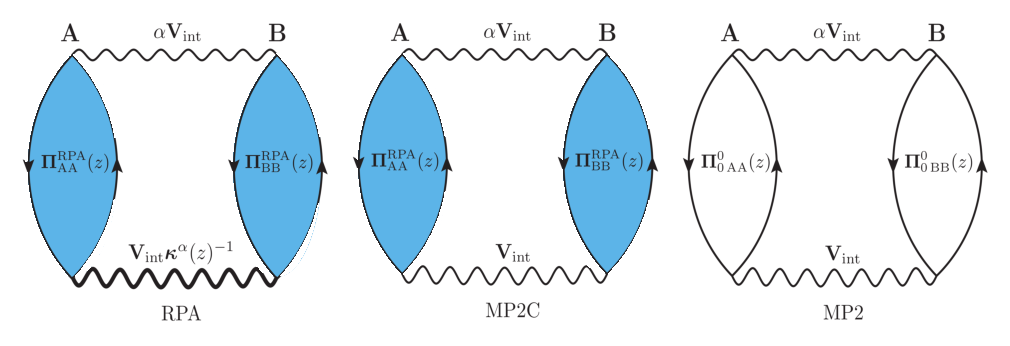
\includegraphics{int_gold_combine.eps}
  \caption{Diagrammatic representations of the A--B dispersion energy
    within RPA, MP2C, and MP2. Blue-shaded and empty rings
    with upward--downward arrows denote particle--hole propagators
    of the monomers containing the full and zero intra-monomer
    interaction, respectively,
    whereas horizontal wavy lines represent interactions between the
    monomers. Coupling strength and frequency integration are
    implied.}
  \label{fig:mp2c_rpa}
\end{figure}

\subsection{Numerical Validation}

\subsubsection{Convergence Estimates}

The previous sections suggest that the AC-SAPT convergence radius
$\alpha_c$ depends critically on the level of theory used to describe
the monomers (through 
$\boldsymbol{\Pi}_0$). Here we numerically evaluate the upper
bounds for 
$\alpha_c^{\text{PT2}}$ and investigate whether these asymptotic bounds
can serve as meaningful convergence estimates for large but finite $R$. 

Starting from Eq. \eqref{eq:alphapt2} and using the same inequalities as in
Sec. \ref{sec:rpa}, we obtain
\begin{equation}
  \alpha_c^{\text{PT2}}(z) \geq \left\| \boldsymbol{\Pi}_0^0(z)
    \mathbf{V}_0 \right\|_2^{-1}.
\end{equation}
Since the spectral norm is invariant under similarity transformations,
\begin{equation}
  \left\| \boldsymbol{\Pi}_0^0(z)
    \mathbf{V}_0 \right\|_2 = \| \mathbf{Q}(z) \|_2,
\end{equation}
where $\mathbf{Q}(z) = -\mathbf{L}^T \boldsymbol{\Pi}^0(z)
\mathbf{L}$ and $\mathbf{L}$ is the Cholesky factor of
$\mathbf{V}^0$. $\mathbf{Q}(z)$ is routinely computed in efficient RPA and beyond-RPA
implementations.\cite{Eshuis10JChemPhys132p234114,Burow14JChemTheoryComput10p180,
doi:10.1021/acs.jctc.8b00777}
For purely imaginary $z$, $\|\mathbf{Q}(z) \|_2$ has a maximum at $z=0$ and
is otherwise monotonous, as may be demonstrated, e.g., using the spectral
representation of $\boldsymbol{\Pi}^0(z)$. Thus, 
\begin{equation}
   \alpha_c^{\text{PT2}}(z) \geq \underline{\alpha}_c^{\text{PT2}} = \|
   \mathbf{Q}(0) \|_2^{-1}.
\end{equation}

\begin{figure}[hbpt]
  \centering
  \includegraphics{eig_q_mp2.eps}
  \caption{Absolute MP2 and RPA interaction energy errors $|\Delta E|$
    for the 
    S66,\cite{doi:10.1021/ct2002946,doi:10.1021/ct200523a}
    L7,\cite{doi:10.1021/ct400036b} and S30L\cite{Sure15JChemTheoryComput}
    benchmarks as well as helium dimer
    as functions of the inverse convergence radius
    $1/\underline{\alpha}_c^{\text{PT2}}$. $\underline{\alpha}_c^{\text{PT2}}$
    was evaluated using a PBE KS reference and cc-pVTZ basis
    sets.}
  \label{fig:eig_q_mp2}
\end{figure}

Figure \ref{fig:eig_q_mp2} shows the correlation between absolute
errors in MP2 interaction energies and the inverse convergence radius $ 
1/\underline{\alpha}_c^{\text{PT2}}$, evaluated
using a PBE KS reference. As long as
$1/\underline{\alpha}_c^{\text{PT2}}$ is close to $1$, the MP2 errors are
small, but they increase rapidly once
$1/\underline{\alpha}_c^{\text{PT2}}$ increases above $\sim 3$. The
correlation is quite convincing since (i) divergence at $\alpha$ values
close to $1$ may not translate into large MP2 errors, (ii) a KS
reference yields $1/\underline{\alpha}_c^{\text{PT2}}$ values 2-3 times
larger than a HF reference, see Fig \ref{fig:eig_q_mp2}. With 
decreasing convergence radius, MP2 and the LHZK(2) dispersion
energy become increasingly incorrect estimates of the exact dispersion
energy \eqref{eq:ecint}. Figure \ref{fig:eig_q_mp2} also shows that the
RPA interaction energies are uncorrelated with
$\underline{\alpha}_c^{\text{PT2}}$, as expected from the estimate
\eqref{eq:alphacrpa}. 

\begin{figure}[hbtp]
  \centering
  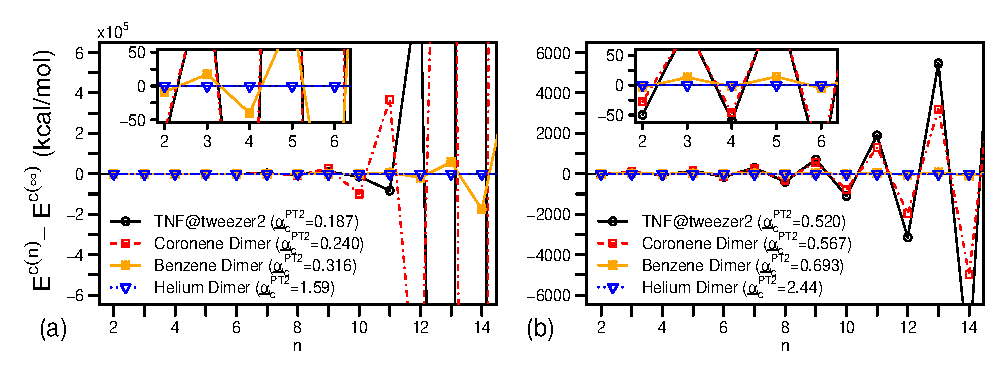
\includegraphics{rpa_expand4.eps}
  \caption{Errors (kcal/mol) of MBPT($n$) interaction energies within
    the ring approximation (i.e. RPA) using (a) a KS and (b) a HF
    reference and cc-pVTZ 
    basis sets. Insets show lower orders on a smaller energy
    scale.} 
  \label{fig:rpa_expand}
\end{figure}

The convergence behavior of the AC-SAPT expansion in relation to
$\underline{\alpha}_c^{\text{PT2}}$
is further illustrated by
re-expansion of the RPA interaction energy in powers of $\alpha$, see
Figure \ref{fig:rpa_expand}. Only for helium dimer
($\underline{\alpha}_c^{\text{PT2}} = 1.59$ with a PBE reference), the
series converges with 
respect to the spectral norm. For all
other cases, increasingly large oscillations are observed at higher
orders. This behavior is characteristic of asymptotic series and has
been observed for MBPT ground state energies.\cite{kato2013perturbation,
  doi:10.1063/1.472352,doi:10.1063/1.481611}
With decreasing $\underline{\alpha}_c^{\text{PT2}}$, the oscillations become
more pronounced lower orders, causing significant error even at
$n=2$. While the convergence radii for some of the smaller systems
are closer to $1$ with a HF reference compared to a PBE reference, their
AC-SAPT series eventually diverge as well.

\begin{figure}[hbpt]
  \centering
  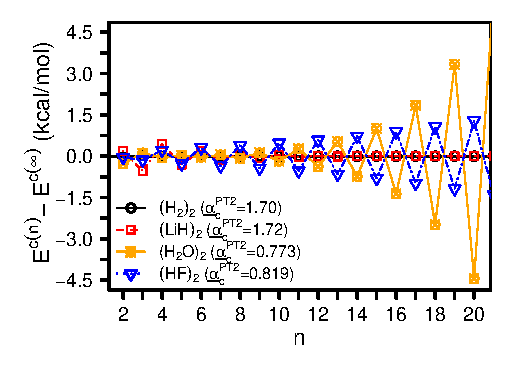
\includegraphics{expand_hf.eps}
  \caption{Errors (kcal/mol) of MBPT($n$) interaction energies within
    the ring approximation (i.e. RPA) using a HF reference and cc-pVTZ
    basis sets for the dimers taken from Ref. \citenum{doi:10.1002/qua.560450502}.}
  \label{fig:hf_expand}
\end{figure}

In their 1993 work\cite{doi:10.1002/qua.560450502}, Moszynski,
Jeziorski, and Szalewicz considered the convergence of MBPT supermolecular
dispersion energies using a HF reference for
He$_2$, (H$_2$)$_2$, (LiH)$_2$, (H$_2$O)$_2$, and (HF)$_2$ within the
ring approximation, which is equivalent to RPA. Based on
numerical results up to order $n=10$, they concluded that the
convergence of the MBPT expansion for these systems is ``very fast.'' 
While we confirm this conclusion for He$_2$, the present results suggest
that the MBPT expansion of the dispersion energy indeed diverges for
modestly larger systems. For example, our results for (H$_2$O)$_2$ agree
well 
with those of Moszynski, Jeziorski, and Szalewicz up to $n=10$, but the
$\underline{\alpha}_c^{\text{PT2}}$ value of 0.773 suggests that the
series is divergent. Indeed, oscillations of increasing magnitude are
observed when orders up to
$n=20$ are considered, see Figure \ref{fig:hf_expand}. 

\subsubsection{Size Dependence of Errors}
\label{subsub:size_dependence}

The dependence of the convergence radius estimate
$\underline{\alpha}_c^{\text{PT2}}$ on the size of the complex is displayed
in Figure \ref{fig:eig_q}. Only for the helium dimer,
$\underline{\alpha}_c^{\text{PT2}} > 1$, whereas
$\underline{\alpha}_c^{\text{PT2}}$ is significantly smaller than $1$
for all systems in the S66,\cite{doi:10.1021/ct2002946,doi:10.1021/ct200523a}
L7,\cite{doi:10.1021/ct400036b} and S30L\cite{Sure15JChemTheoryComput}
benchmarks. Clearly, as opposed to $\boldsymbol{\Pi}_0^{\text{RPA}}(0)$,
$\boldsymbol{\Pi}^0(0)$ is not necessarily bounded. Whether $\| \boldsymbol{\Pi}^0(0)
\mathbf{V}_{\text{int}} \|_2$ saturates or becomes infinite in the
thermodynamic limit is system-dependent;
nevertheless, the convergence criterion Eq.~\eqref{eq:conv} suggests that
perturbative calculations of NIs start to diverge already for
fairly small system sizes with few tens of atoms and comparatively large
HOMO--LUMO gap. Indeed, the HOMO--LUMO gap is a fairly poor estimator of
the interaction energy error, see Supporting Information. 

\begin{figure}[hbpt]
  \centering
  \includegraphics{eig_q.eps}
  \caption{Inverse of the convergence radius
    ($1/\underline{\alpha}_c^{\text{PT2}}$) for MBPT(2) with PBE and HF
    references vs. number of valence 
    electrons (VEs) for the
    S66,\cite{doi:10.1021/ct2002946,doi:10.1021/ct200523a} 
    L7,\cite{doi:10.1021/ct400036b} and S30L
    \cite{Sure15JChemTheoryComput} benchmarks, and helium dimer.
    $\underline{\alpha}_c^{\text{PT2}}$ values were computed using
    cc-pVTZ basis sets. A $1/\underline{\alpha}_c^{\text{PT2}}$ value
    $\ge 1$ indicates divergence of the AC-SAPT series.} 
  \label{fig:eig_q}
\end{figure}

Relative errors in NIs as a function of system size are shown in
Figure \ref{fig:mp2_rpa_comp}. While the correlation of the errors with
the number of valence electrons (VEs) is
less strong than the one observed for the convergence estimates, there
are clearly discernible trends: Whereas percentage errors in binding
energies are virtually constant within RPA, they increase linearly for
MP2, at a rate of approximately 0.1$\%$, per VE
on average. For slightly over 700 valence electrons, the MP2 relative error 
regression fit reaches 100\% for the systems tested here. SCS-MP2 has an
approximately 5 times lower slope of 0.025$\%$, per VE
(but notably higher y-intercept), and PBE-D3 relative errors grow
at a rate of slightly less than 0.01$\%$, for the present
benchmarks, see Table \ref{tab:slopes}. The largest MP2 errors occur for
systems with strong $\pi$--$\pi$ stacking interactions such as complexes 3
to 12 from the S30L test set.\cite{Sure15JChemTheoryComput}

\begin{figure}[hbpt]
  \centering
  \includegraphics{mp2_rpa_signed.eps}
  \caption{Relative errors ($\Delta E$) of MP2, SCS-MP2, RPA(PBE), and
    PBE-D3 interaction energies in the
    S66,\cite{doi:10.1021/ct2002946,doi:10.1021/ct200523a} 
    L7,\cite{doi:10.1021/ct400036b} and
    S30L\cite{Sure15JChemTheoryComput} benchmarks vs.
    number of valence electrons (VEs).}
  \label{fig:mp2_rpa_comp}
\end{figure}

\begin{table}[hbpt]
  \caption{Parameters of the linear regression
    fits displayed in Figure \ref{fig:mp2_rpa_comp}. The slope
    corresponds to the 
    average relative interaction energy error ($\%$) per valence electron (VE), and
    the $y$-intercept corresponds to the average relative interaction
    energy error ($\%$) in the limit of zero VEs.} 
  \begin{tabular}{lRR}
    \hline
    \text{Method} & \text{Slope ($\%$/VE)} & y\text{-intercept (\%)} \\
    \hline
    \text{MP2} & 0.1219 & 7.30 \\
    \text{SCS-MP2} & 0.0251 & 14.10 \\
    \text{RPA(PBE)}& 0.0030 & 6.24 \\
    \text{PBE-D3}  & 0.0083 & 6.79 \\
    \hline
  \end{tabular}
  \label{tab:slopes}
\end{table}

\subsection{Physical Interpretation}

The present analytical and numerical results show that the convergence
of the AC-SAPT series for NIs is strongly dependent on the level of theory
used for computing the monomer polarization propagator
$\boldsymbol{\Pi}^0(z)$. Thus, it is helpful to consider the generalized
dielectric function
\begin{equation}
    \boldsymbol{\epsilon}_0(z) = \mathbf{1} - \boldsymbol{\Pi}^0(z)
  \mathbf{V}_0,
\end{equation}
which characterizes the response of the monomers at frequency
$z$. Within RPA, Eq. \eqref{eq:rpabound} implies that the 
eigenvalues of $\boldsymbol{\epsilon}_{0}$ are bounded from above by
$2$, reflecting the fact that the RPA response to external fields is
reduced (``screened'') by the creation of induced electron-pairs. As a
result, the 
effective interaction ``seen'' by an electron of subsystem A due to
electrons in subsystem B decays rapidly within B. This effective
interaction is indeed ``weak'' in the sense that 
it affords a convergent AC-SAPT expansion for nondegenerate monomers.

For systems satisfying the DG conditions, there is no screening in the
monomers in at least one dimension, and the largest eigenvalue of
$\boldsymbol{\epsilon}_{0}(z)$ may equal 2, even within RPA, causing
divergence of the AC-SAPT expansion and unconventional power laws of the
dispersion interaction. Since the HXC kernel is dominated by the Hartree
kernel for large $R$, this behavior of the RPA is expected to be
correct, at least qualitatively.

As opposed to these physical divergences of the AC-SAPT expansion,
unphysical divergences may result if the intra-monomer electron
interaction is treated perturbatively. In this case, 
$\boldsymbol{\epsilon}_{0}$ is not bounded, with largest eigenvalues
around 5 (KS reference) or 2 (HF reference) for typical systems studied
here, see Figures \ref{fig:eig_q_mp2} and \ref{fig:eig_q}. This reflects
a much stronger perturbation of the monomers by the intersystem
interaction due to incomplete screening resulting primarily from the
neglect of higher-order particle--hole ring diagrams. Hence, the MBPT
effective interaction is too strong for intermolecular perturbation
theory, causing spurious divergence of the AC-SAPT expansion. This effect
is not seen in the smallest and least polarizable monomers 
such as He atoms, but it becomes noticeable for even moderately large
monomers with a few atoms, where the neglect of screening due to
multiple induced particle--hole pairs by finite-order MBPT produces
significant over- or underestimations of NIs. For the large $\pi$
systems in the S30L, the lack of screening produces maximum eigenvalues
of $\boldsymbol{\epsilon}_{0}$ around 7 (KS reference) or 3 (HF
reference), which suggests rapid divergence of the AC-SAPT expansion,
providing a plausible rationale for the spectacular errors in MP2
binding energies observed for these systems.

\section{Conclusions}
\label{sec:conclusions}

A key result of this study is that dispersion interactions cannot be
considered ``weak'' unless intra-monomer screening effects are taken
into account at least at the level of RPA. Similar to electrostatic
screening, electrodynamic screening due to induced density fluctuations is
inadequately captured by finite-order MBPT-type approaches, except for the
smallest and least polarizable systems. As a result, unscreened
perturbation theories 
produce exaggerated responses of the monomers to external perturbation and 
divergent estimates for NIs even in moderately large systems. The
conventional 
wisdom that MBPT is useful for accurate calculations of NIs in even
moderately large systems is incorrect: Numerically small interaction
energies compared to covalent interactions do not imply ``weakness'' in
the sense of a bounded response or convergent intermolecular perturbation
theory. Consequently, finite-order MBPT results tend to worsen systematically
with system size, as was demonstrated by the basis-set extrapolated MP2 results
for complexes with up to 600 VEs. Given the computational
efficiency and popularity of MBPT implementations, this is a sobering result:
Size-extensivity and (conventional) size-consistency are insufficient
conditions for accurate predictions of NIs. While there may
be a place for MBPT calculations of NIs in complexes of small,
hard monomers, MBPT estimates of NIs cannot be considered
reliable for most systems of chemical interest, much less for nanomaterials,
metallic systems, or soft matter. In light of the current results,
empirically scaled MP2 methods, and particularly MP2.5, appear as
simple regularizations of an asymptotic series; while this strategy is
clearly successful for some systems, it does not address the underlying
physical problem, limiting predictive power and robustness.

The MP2C
method can be viewed as a partial MBPT resummation which includes
intramonomer screening and exhibits better analytical properties than
bare MBPT, but
truncates intermonomer interactions at second order, and has no obvious
supermolecular 
equivalent. For increasingly large and polarizable monomers, MP2C
underestimates the magnitude of dispersion interactions 
progressively due to missing many-body dispersion.

A qualitatively correct treatment of intra-monomer
screening to all orders is possible with RPA at little extra cost
compared to MBPT approaches. Indeed, RPA produces
constant relative errors in NIs that are virtually independent of the system
size and type, consistent with its qualitatively correct treatment of
electrodynamic 
polarization; this may be viewed as a manifestation of ``Casimir-Polder
size consistency.''\cite{doi:10.1021/acs.jctc.7b00996}
Similar conclusions may hold for more elaborate 
non-perturbative coupled cluster methods, which include the ring
diagrams corresponding to RPA.\cite{doi:10.1063/1.3043729}
In particular, the accuracy of ring-coupled-cluster methods for
NIs\cite{doi:10.1063/1.3626551}
supports the view that ring diagrams dominate in the long-range limit
of NIs. It is remarkable that ring diagrams also constitute the main part
of the correlation energy for the uniform electron gas at high
density,\cite{PhysRev.106.364} 
a similarity first noted by Dzyaloshinskii, Lifshitz, and
Pitaevskii.\cite{Dzyaloshinskii1961165} Both, dispersion interactions in
finite systems and electron correlation in the high-density electron gas
emerge from collective density fluctuations\cite{PhysRev.82.625,PhysRev.85.338}
caused by the long-range Coulomb interaction. In this sense, the expectation
that RPA energy differences should be universally accurate\cite{PhysRevB.61.16430,PhysRevB.81.169902}
appears to hold as long as long-range correlation dominates. 

The present results raise the question whether the perturbative triples
correction of CCSD(T) inherits any of the limitations of MBPT, even though it
includes some screening at the level of the amplitudes. Whereas CCSD(T)
errors for interaction energies of small molecular complexes were determined
to be on the order of 1\%,\cite{doi:10.1021/ct400036b} and typical deviations
between RPA and CCSD(T) binding energies are on the order of 5-10\% for
the benchmarks studied here, the linear scaling domain-based pair natural
orbital CCSD(T) binding energies for water on small graphene flakes are
significantly larger than the corresponding RPA and diffusion Monte Carlo
ones,\cite{doi:10.1021/acs.jctc.9b00110} and the CCSD(T) perturbative triples
correction diverges for the correlation energy of the uniform electron
gas.\cite{PhysRevLett.110.226401}

The AC-SAPT formalism developed here affords separate, non-perturbative
definitions of dispersion and induction effects in NIs. While it has
mainly been used to rationalize the results of supermolecular
calculations here, the analytical expressions obtained from AC-SAPT
could be evaluated using monomer calculations given suitable
approximations to the intermolecular KS potential
$\hat{V}_{s\,\text{int}}[\rho]$. Beyond-RPA perturbation
methods known from supermolecular calculations such as
second-order screened exchange
(SOSEX)\cite{doi:10.1063/1.3250347,doi:10.1063/1.3317437,doi:10.1063/1.3501928,
doi:10.1063/1.5025938}
or approximate exchange kernel (AXK)\cite{Bates13JChemPhys139p171103,doi:10.1021/acs.jctc.8b00777}
may prove useful for this purpose. Our
conclusions regarding the divergence of MBPT for NIs rely in part on the
assumption that the RPA dispersion energy is qualitatively accurate, which is
supported by the close agreement between the RPA and the benchmark results.
This agreement is remarkable given that RPA is parameter-free aside from
using a KS reference from a semilocal DFA. Moreover, the estimated
AC-SAPT convergence radii are upper bounds only, but they show strong
correlation to the NI errors of MBPT methods for the benchmarks studied
here.

Our results show that the convergence of the AC-SAPT expansion for
dimers consisting of large monomers depends critically on the accuracy
of intra-monomer correlation. Specifically, electrodynamic 
screening should be included in the monomer correlation treatment at
least at the time-dependent HF level. Apart from unphysical
divergences, AC-SAPT does converge more slowly for large and polarizable
monomers, and exhibits physical divergence for systems satisfying
the DG conditions such as one-dimensional metals. Under these circumstances,
the traditional  LHZK(2) picture of dispersion breaks down and must
replaced by the RPA one embodied in Eq.~\eqref{eq:ecabrpa}. Importantly,
Eq.~\eqref{eq:ecabrpa} correctly recovers both, the small, hard
monomer LHZK(2) limit where MBPT can converge, and the
macroscopic Lifshitz limit. Eq.~\eqref{eq:ecabrpa} is largely scale
invariant and therefore a far better starting point for computing
and conceptualizing dispersion interactions than LHZK(2).

The breakdown of MBPT for NIs also has important implications for the
development of approximations such as van-der-Waals density functionals
or force fields. The present results cast further doubt on the validity of
empirical $1/R^6$ corrections for very large and polarizable monomers --
even though some dispersion-corrected DFAs admittedly perform remarkably
well for large systems.
An accurate description of NIs for such systems may require methods including
Lifshitz-type physics and electrodynamic polarization effects. Quantum
Drude models\cite{PhysRevB.87.144103} or many-body dispersion
methods\cite{Tkatchenko12PhysRevLett108p236402,doi:10.1021/acs.chemrev.6b00446}
may be considered coarse-grained RPA approaches suitable for this purpose. 

Modern RPA implementations are insignificantly more expensive than the
most advanced MP2 approaches from a computational viewpoint, and RPA
calculations for molecules with 
hundreds of atoms on workstation clusters are now routine
\cite{Eshuis10JChemPhys132p234114,Hesselmann12PhysRevA85p012517,Riplinger13JChemPhys,   
  Kallay15JChemPhys142p204105,Chen17AnnuRevPhysChem68p421,Schurkus16JChemPhys144p031101,
  doi:10.1021/acs.jctc.6b01235,doi:10.1063/1.5052572,doi:10.1021/acs.jctc.9b00444}
--- although the present results also show that accurate RPA binding
energies for NIs require triple- to quadruple-$\zeta$ basis set
extrapolation, making some of the proposed low-scaling methods less 
effective. 
Taken together with the superior accuracy of RPA for large and polarizable
systems without empirical adjustments, MP2 can be safely and efficiently
replaced by RPA for calculations of NIs in most systems of chemical
interest. If MP2 results are nevertheless desired,
diagnostic $\underline{\alpha}_{c}^{\text{PT2}}$ values should be
used to gauge their reliability. Similarly, the present results support
the use of RPA calculations to calibrate dispersion-corrected DFA results.

RPA calculations of NIs benefit from variational
optimization of the reference \cite{PhysRevA.99.012518}, but the
improvement appears to be most pronounced for small systems such as rare
gas dimers and diminish with increasing monomer size. With average interaction
energy errors consistently in the 5--10\% range, RPA is accurate enough for
a wide range of applications, irrespective of system size, gap size, or empirical
training sets. The accuracy of RPA for NIs may also contribute to its
recent successful application to activation energies of sterically
crowded transition
states.\cite{Tao16ChemEurJ22p8786,doi:10.1021/acs.joc.9b01319} 

%%%%%%%%%%%%%%%%%%%%%%%%%%%%%%%%%%%%%%%%%%%%%%%%%%%%%%%%%%%%%%%%%%%%%
%% The "Acknowledgement" section can be given in all manuscript
%% classes.  This should be given within the "acknowledgement"
%% environment, which will make the correct section or running title.
%%%%%%%%%%%%%%%%%%%%%%%%%%%%%%%%%%%%%%%%%%%%%%%%%%%%%%%%%%%%%%%%%%%%%
\begin{acknowledgement}
  
This material is based upon work supported by
the National Science Foundation under CHE-1464828 and CHE-1800431.

The authors declare the following competing financial interest(s):
Principal investigator Filipp Furche has an equity interest in Turbomole
GmbH. The terms of this arrangement have been reviewed and approved by
the University of California, Irvine, in accordance with its conflict of
interest policies.

\end{acknowledgement}

%%%%%%%%%%%%%%%%%%%%%%%%%%%%%%%%%%%%%%%%%%%%%%%%%%%%%%%%%%%%%%%%%%%%%
%% The same is true for Supporting Information, which should use the
%% suppinfo environment.
%%%%%%%%%%%%%%%%%%%%%%%%%%%%%%%%%%%%%%%%%%%%%%%%%%%%%%%%%%%%%%%%%%%%%
\begin{suppinfo}

A listing of the contents of each file supplied as Supporting Information
should be included. For instructions on what should be included in the
Supporting Information as well as how to prepare this material for
publications, refer to the journal's Instructions for Authors.

The following files are available free of charge:
\begin{itemize}
\item si.pdf: Total energies for the L7, S30L, and S66 benchmarks,
  complete ROT34 results, and further details and results
\end{itemize}

\end{suppinfo}

%%%%%%%%%%%%%%%%%%%%%%%%%%%%%%%%%%%%%%%%%%%%%%%%%%%%%%%%%%%%%%%%%%%%%
%% The appropriate \bibliography command should be placed here.
%% Notice that the class file automatically sets \bibliographystyle
%% and also names the section correctly.
%%%%%%%%%%%%%%%%%%%%%%%%%%%%%%%%%%%%%%%%%%%%%%%%%%%%%%%%%%%%%%%%%%%%%
\bibliography{references}

\end{document}
